\chapter[Resultados dos experimentos e discussão]{Resultados dos experimentos e discussão}

%%%%
%
% Gerador de tabelas: http://www.tablesgenerator.com/
%
% Elementos: http://www.tutorbrasil.com.br/forum/viewtopic.php?t=6163
%
% Sinônimos-> Assim sendo
% então, por conseguinte, deste jeito, desta maneira, dessarte, dessa forma, deste modo, desta forma, sendo assim, consequentemente, por isso, destarte, assim, portanto, logo, isto posto.
%
%
%%%%

Neste capítulo, avaliamos os impactos resultantes da remoção dos genes sementes nas listas de priorização resultante em comparação com a lista original. 
%
Ou seja, o quanto a lista de genes resultantes foram recuperados nos experimentos com remoção das sementes em relação a lista resultante original.

Conforme mencionado no capítulo anterior, realizamos experimentos mantendo fixos a rede PPI e os dados de expressão, mas removendo progressivamente parte dos nós sementes do conjunto original (de forma similar as técnicas de avaliação de classificadores \textsl{leave-one-out} e validação cruzada), e comparando a interseção entre seus resultados com o resultado original.
Após isso, variamos o percentual de genes sementes excluídos entre 10\% e 40\% e, em seguida, comparamos os primeiros elementos das listas resultantes com os primeiros da lista original. 


%
%===================== MEDIDAS DE CENTRALIDADE ===================
%

\section{Medidas de centralidade dos genes sementes}

Primeiramente, uma importante questão a ser verificada é se o impacto causado nos resultados devido à remoção de alguns genes sementes está correlacionado com alguma medida de centralidades dos respectivos genes na rede PPI.
Em outras palavras, tais medidas podem informar se o impacto da remoção dos genes sementes deve-se predominantemente a fatores topológicos.
%
A Tabela~\ref{centrality_measures} apresenta as medidas de centralidade que os genes sementes utilizados possuem na rede PPI.
Os genes estão apresentados ordenados pelo grau decrescente.
Observamos que os três primeiros genes: \textsl{TP53} (333), \textsl{AKT1} (138) e \textsl{DISC1} (91), possuem grau destacadamente maior que os demais, que possuem grau abaixo de 50.

% ============= Tabela com medidas de centralidade =========
\begin{table}[]
\centering
\caption{Medidas de centralidade dos genes sementes utilizados no experimento}
\label{centrality_measures}
\footnotesize
\begin{tabular}{@{}lrrrrrrr@{}}
\toprule
\textbf{\textsl{GENE}} & \textbf{Degree} &   \textbf{Betweenness} & \textbf{Closeness} & \textbf{Clustering} & \textbf{Brokering}  & \textbf{Bridgeness} \\ \midrule
\textbf{\textsl{TP53}}  & 333 & 1017443.366745 & 0.401408 & 0.027968 & 0.034839 &  135.635614 \\
\textbf{\textsl{AKT1}}  & 138 &  260150.217669 & 0.374562 & 0.044219 & 0.014196 &  206.018081 \\
\textbf{\textsl{DISC1}}  &  91 &  131642.895006 & 0.333142 & 0.016606 & 0.009632 &  130.539882 \\
\textbf{\textsl{FEZ1}}  &  43 &   39961.948306 & 0.315902 & 0.024363 & 0.004515 &  196.253855 \\
\textbf{\textsl{ERBB4}}  &  40 &   21172.397911 & 0.325737 & 0.144872 & 0.003682 &  188.374839 \\
\textbf{\textsl{GRIN2B}}  &  33 &   23614.446663 & 0.317337 & 0.090909 & 0.003229 &  362.909288 \\
\textbf{\textsl{APOE}}  &  29 &   19099.496744 & 0.318884 & 0.088670 & 0.002845 &  346.398103 \\
\textbf{\textsl{HP}}  &  21 &   22059.197543 & 0.324588 & 0.047619 & 0.002153 &  519.171834 \\
\textbf{\textsl{DRD2}}  &  17 &   15283.833355 & 0.301050 & 0.014706 & 0.001803 &  580.045729 \\
\textbf{\textsl{HTR2A}}  &  16 &    5847.333317 & 0.292464 & 0.008333 & 0.001708 &  212.879317 \\
\textbf{\textsl{IL1B}}  &  10 &    8530.925938 & 0.304214 & 0.066667 & 0.001005 & 1381.703074 \\
\textbf{\textsl{RGS4}}  &  10 &    2039.400569 & 0.292253 & 0.066667 & 0.001005 &  463.743523 \\
\textbf{\textsl{GAD1}}  &  10 &    7993.469172 & 0.317012 & 0.222222 & 0.000837 &  888.443883 \\
\textbf{\textsl{DRD1}}  &   8 &    9964.681533 & 0.282170 & 0.071429 & 0.000800 &  827.421927 \\
\textbf{\textsl{PPP3CC}}  &   8 &   10512.488952 & 0.289196 & 0.035714 & 0.000830 &  985.201738 \\
\textbf{\textsl{NRG1}}  &   7 &     349.958475 & 0.272072 & 0.238095 & 0.000574 &  126.388843 \\
\textbf{\textsl{COMT}}  &   5 &    3676.951004 & 0.273329 & 0.000000 & 0.000538 & 1028.239964 \\
\textbf{\textsl{SLC6A4}}  &   5 &     565.928439 & 0.283911 & 0.000000 & 0.000538 &  197.019715 \\
\textbf{\textsl{DRD4}}  &   5 &    2814.994398 & 0.298228 & 0.000000 & 0.000538 & 1209.842385 \\
\textbf{\textsl{PLXNA2}}  &   4 &    9316.180826 & 0.264610 & 0.000000 & 0.000431 & 1746.023442 \\
\textbf{\textsl{TPH1}}  &   4 &     574.162877 & 0.312481 & 0.333333 & 0.000287 & 7943.713227 \\
\textbf{\textsl{RELN}}  &   4 &      43.733810 & 0.240987 & 0.333333 & 0.000287 &   13.904311 \\
\textbf{\textsl{GRM3}}  &   4 &     248.812705 & 0.284468 & 0.000000 & 0.000431 &  597.497122 \\
\textbf{\textsl{GABRB2}}  &   4 &     555.585080 & 0.261145 & 0.000000 & 0.000431 &  288.445351 \\
\textbf{\textsl{DAO}}  &   3 &     768.669783 & 0.283496 & 0.000000 & 0.000323 &  676.604177 \\
\textbf{\textsl{OPCML}}  &   1 &       0.000000 & 0.253044 & 0.000000 & 0.000108 &    0.000000 \\
\textbf{\textsl{ZNF804A}}  &   1 &       0.000000 & 0.258773 & 0.000000 & 0.000108 &    0.000000 \\
\textbf{\textsl{MTHFR}}  &   1 &       0.000000 & 0.238457 & 0.000000 & 0.000108 &    0.000000 \\
\textbf{\textsl{RPGRIP1L}}  &   1 &       0.000000 & 0.270930 & 0.000000 & 0.000108 &    0.000000 \\
\textbf{\textsl{GRIK4}}  &   1 &       0.000000 & 0.229498 & 0.000000 & 0.000108 &    0.000000 \\ \bottomrule

\end{tabular}
\flushleft{Fonte: Tabela gerada pelo autor.}
\end{table}

% ========== FIM TABELA DE MEDIDAS DE CENTRALIDADE



\section{Remoção de um único gene semente}
%
Inicialmente, avaliamos o impacto da remoção de um único gene semente na lista resultante.
Esta avaliação foi realizada de forma similar ao método \textit{Leave-One-Out Cross-Validation}.
A ideia deste experimento foi avaliar o impacto individual de cada gene no resultado final, com relação aos dois escores $X$ e $\Delta'$, obtidos durante a análise da rede diferencial no método \textsl{NERI}.
Em seguida, comparamos o impacto de tais resultados com as medidas de centralidade de redes para avaliar se há alguma correlação.
Desta forma, esta informação pode ser utilizada para lançar luz sobre o impacto das remoções de múltiplos genes sementes.

\subsection{Estudo dos gráficos em relação ao escore $\Delta'$}
%
% ============== S ===============
%
\subsubsection{Análise dos 10 primeiros elementos}
A figura \ref{fig_LOO_S_10} apresenta um gráfico comparativo dos experimentos utilizando o método de \textit{remoção de um único gene}, onde o eixo \textit{Horizontal} representa o gene removido em relação a amostra original, e o eixo \textit{Vertical}, por sua vez, representa a diferença percentual dos genes ranqueados em relação ao experimento original. Desta forma, comparando os 10 primeiros genes ranqueados relativos a remoção de cada gene apresentado, em relação aos 10 primeiros apresentados na amostra original, sendo o fator de ranqueamento o escore $\Delta'$.
%
%Imagem
\begin{figure}[ht!]
\centering
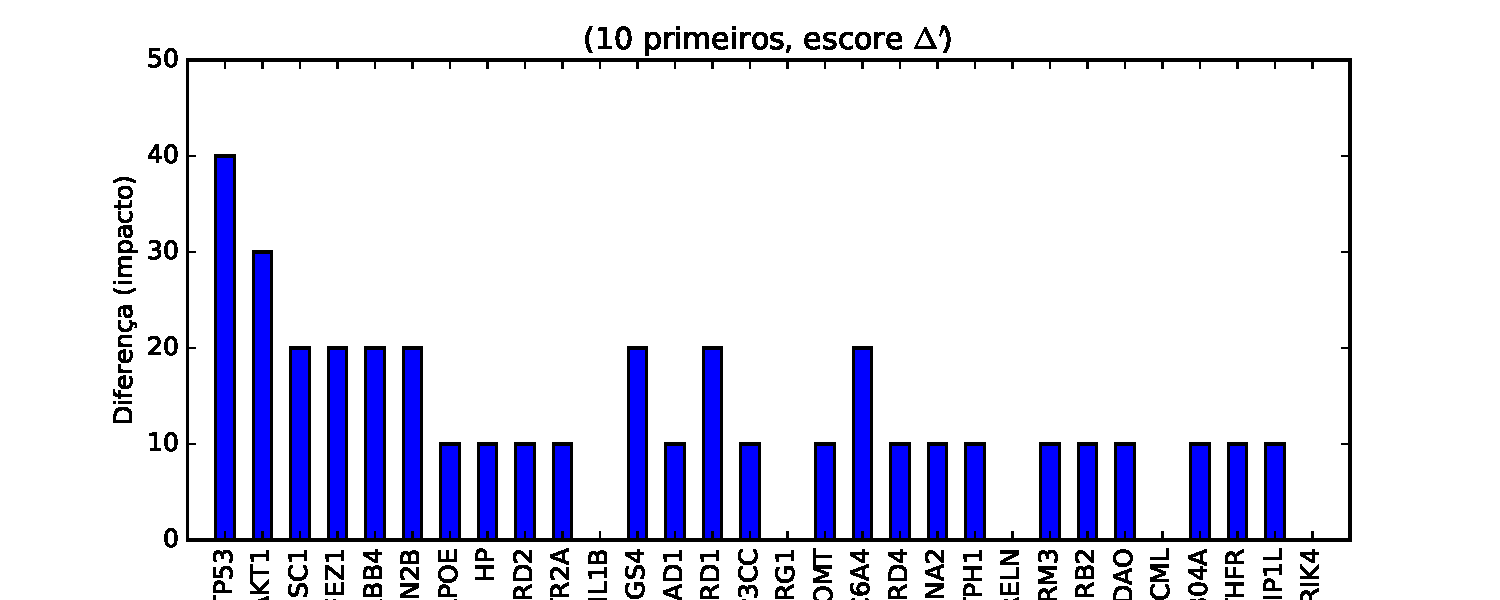
\includegraphics[width=\textwidth]{Images/analyses/fig_LOO_S_10.pdf}
\caption {Análise dos 10 primeiros elementos ordenados por $\Delta'$.
\label{fig_LOO_S_10}}
\flushleft{Fonte: Produzido pelos autores.}
\end{figure}
%

Podemos observar que os genes de maior grau \textbf{\textit{TP53}} (333) e \textbf{\textit{AKT1}} (138), apresentaram impactos um pouco maior que os demais que foram respectivamente de \textbf{\textit{40\%}} e \textbf{\textit{30\%}}.
No entanto, ao comparar com o impacto dos demais genes que não têm graus tão altos, observamos que, de uma forma geral, os impactos não foram diretamente proporcionais aos graus dos genes.
%

Observamos também que os genes \textbf{\textit{IL1B, RELN, NRG1, GRIK4}} e \textbf{\textit{OPCML}} não apresentaram mudanças no resultado em relação ao escore analisada ($\Delta'$), assim como o gene \textbf{\textit{MTHFR}} e os outros que apresentaram \textbf{\textit{10\%}} de diferença dos genes selecionados, comparado ao resultado original do experimento.
Devido a isto, podemos presumir de que tais genes não apresentam uma importância significativa para o método em estudo em relação aos 10 primeiros selecionados utilizando o fator de ranqueamento o escore $\Delta'$.
%

Os genes \textbf{\textit{CHRNA7, DAOA, DTNBP1, MUTED, NPAS3, OFCC1, PRODH}} e \textbf{\textit{SLC18A1}} não foram integrados com a rede PPI.
Ou seja, durante a integração de dados, tais genes não possuíam um nó correspondente na rede PPI e, portanto, não foram utilizados.

Ao analisar os genes mencionados anteriormente \textbf{\textit{TP53}} e \textbf{\textit{AKT1}}, ambos possuem um alto grau na rede gerada pelo método NERI.
E isto pode sugerir que a remoção de um gene com alto grau influencia diretamente no resultado.
%
Por outro lado, os demais genes deram valores bastante parecidos, oscilando entre 0\% à 10\%.
Por exemplo, os genes \textsl{\textbf{ZNF804A}}, \textsl{\textbf{MTHFR}} e \textsl{\textbf{RPGRIP1L}} possuem grau \textsl{\textbf{1}}, e no entanto, causaram \textsl{10\%} de impacto em relação ao experimento original, onde apresenta-se semelhante a remoção do terceiro gene, o \textsl{\textbf{DISC1}} com grau \textsl{91}.
Isso demonstra que a correlação entre o grau e o impacto observado na lista resultante final não é direta. 
%

%
\subsubsection{Análise dos 20 e 50 primeiros elementos}
%
%Imagem
\begin{figure}[ht!]
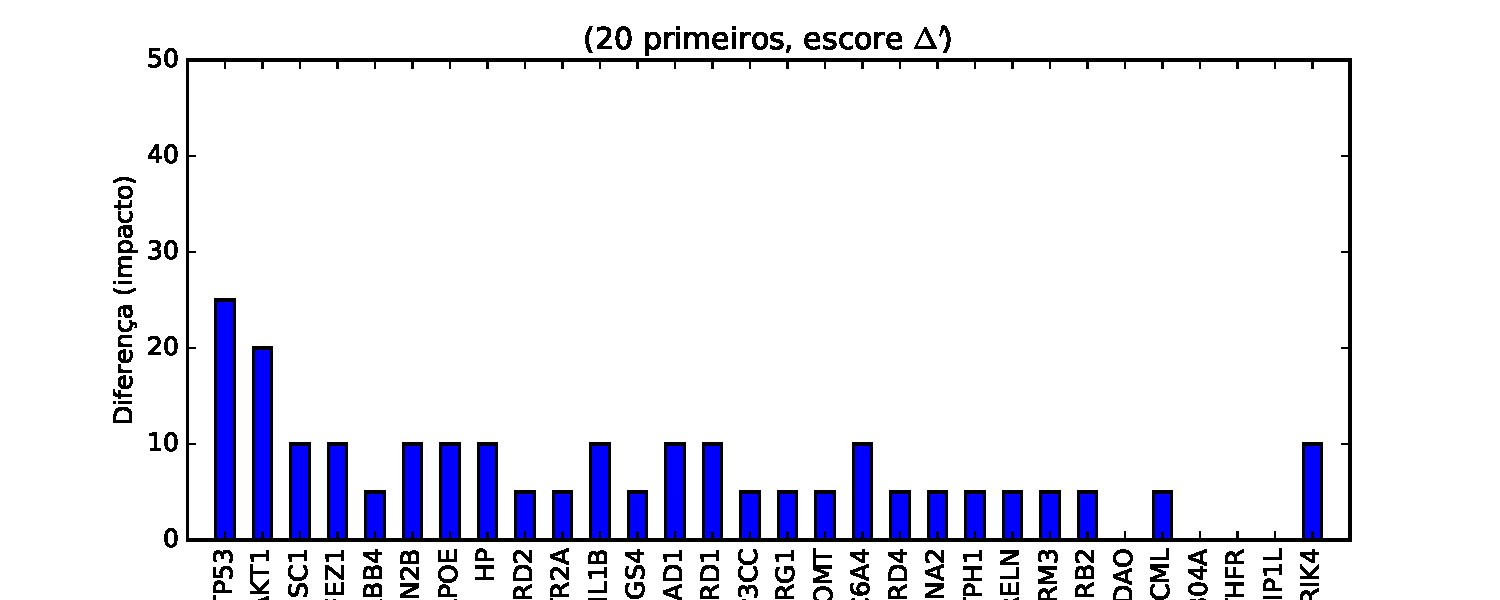
\includegraphics[width=1\textwidth]{Images/analyses/fig_LOO_S_20.pdf}
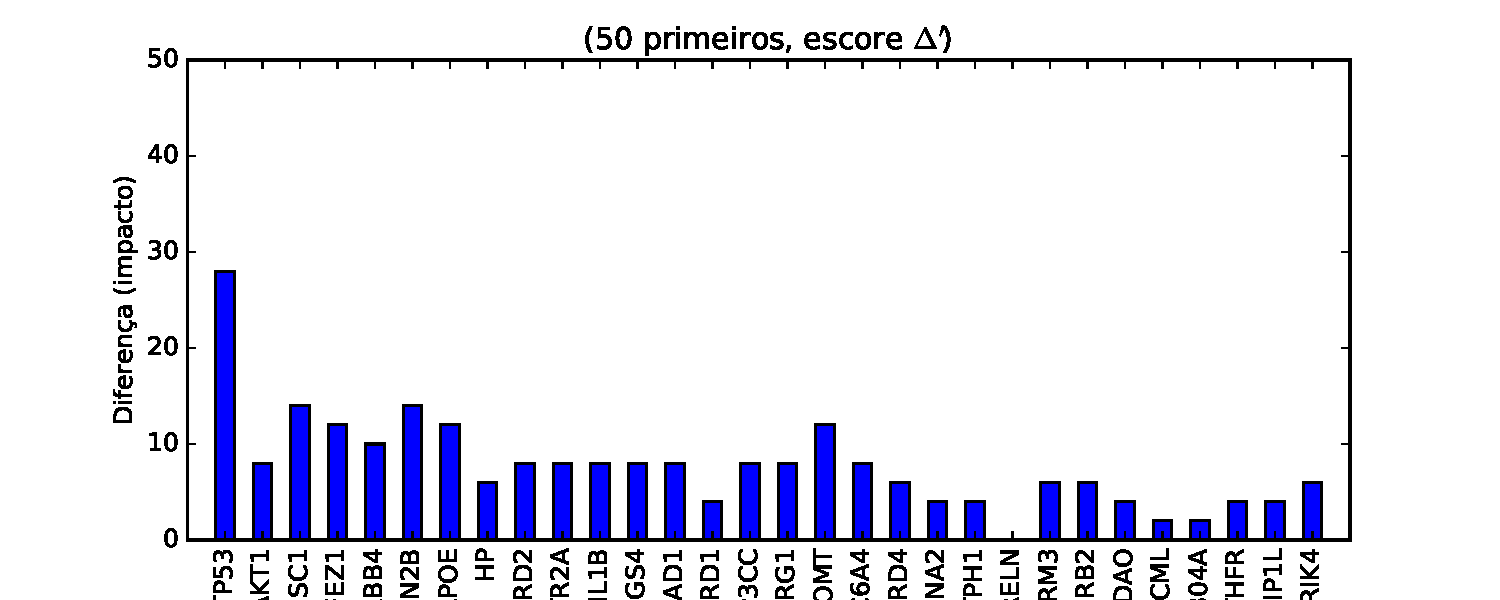
\includegraphics[width=1\textwidth]{Images/analyses/fig_LOO_S_50.pdf}
\caption {Análise dos 20 e 50 primeiros elementos ordenados por $\Delta'$.
\label{fig_LOO_S_20-50}}
\flushleft{Fonte: Produzido pelos autores.}
\end{figure}
%

A figura \ref{fig_LOO_S_20-50} apresenta dois gráficos de forma comparativa, de modo que o de cima representa os \textbf{\textit{20}} primeiros genes ranqueados resultantes em relação ao escore $\Delta'$ e o gráfico de baixo apresenta os \textbf{\texit{50}} primeiros. Sendo eixo \textit{Vertical} a similaridade com o resultado original e o eixo \textit{Horizontal} o gene removido no experimento em questão.
%

A remoção do gene \textbf{\texit{MTHFR}} apresentou baixo impacto: \textbf{\textit{0\%}} de diferença nos primeiros \textbf{\textit{20}} elementos e  \textbf{\textit{5\%}} em relação aos primeiros \textbf{\textit{50}} elementos da lista original.
%
Este mesmo efeito aconteceu na remoção do gene \textbf{\textit{RELN}}, variando de \textbf{\textit{0\%}} de diferença percentual, dos genes selecionados em relação ao experimento original, nos primeiros \textbf{\textit{20}} elementos para \textbf{\textit{5\%}} em relação aos primeiros \textbf{\textit{50}}.
%

Podemos observar também uma diminuição de experimentos com \textbf{\textit{10\%}} ou menos de impacto. Caindo de \textbf{\textit{36}} experimentos ao todo e \textbf{\textit{28}} válidos, para \textbf{\textit{31}} ao todo e \textbf{\textit{23}} válidos (Os experimentos não válidos para análise são os que não integraram com a base de dados \textbf{\textit{GWAS}}, totalizando \textbf{\textit{8}} \textit{genes/experimentos}).
%

O gene \textbf{\textit{TP53}} que causa o maior impacto na similaridade em sua remoção, variou de \textbf{\textit{25\%}} para \textbf{\textit{29\%}} nos respectivos agrupamentos \textbf{\textit{20}} e \textbf{\textit{50}} primeiros genes selecionados. Isso implica que ao analisar \textbf{\textit{30}} elementos a mais, houve um aumento do impacto de \textbf{\textit{4\%}} no pior caso. Sugerindo uma boa robustez do método em relação a remoção de um único gene semente.
%

Outro ponto importante de observação, é o gene \textsl{\textbf{AKT1}} que possui um alto grau na rede gerada pelo método NERI, apresentar uma variação de impacto no resultado bem alta. O impacto apresentado vai de \textsl{\textbf{20\%}} para \textsl{\textbf{8\%}}, nos gráficos representantes dos \textsl{\textbf{20}} e \textsl{\textbf{50}} primeiros genes, respectivamente.
Este fator aponta, mais um vez, que o grau do gene relativo a rede não causa um impacto diretamente proporcional ao grau.

%
\subsubsection{Análise dos 100 e 200 primeiros elementos}
%
%Imagem
\begin{figure}[ht!]
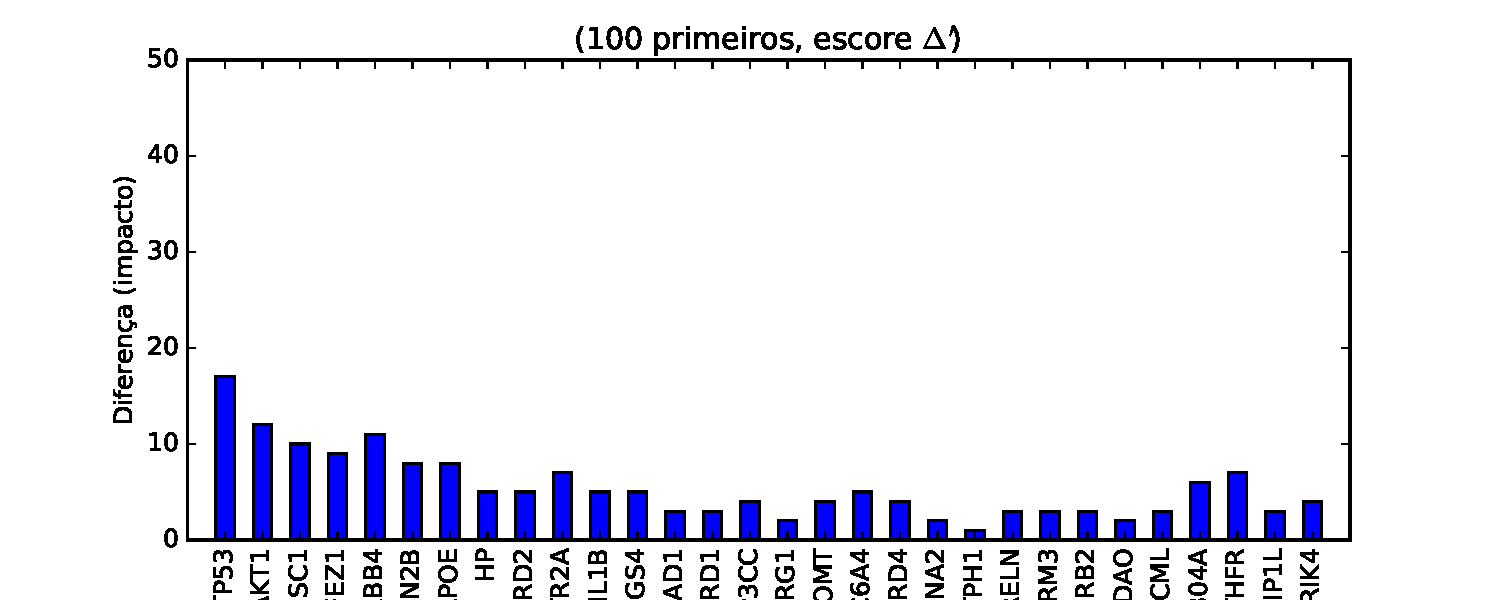
\includegraphics[width=1\textwidth]{Images/analyses/fig_LOO_S_100.pdf}
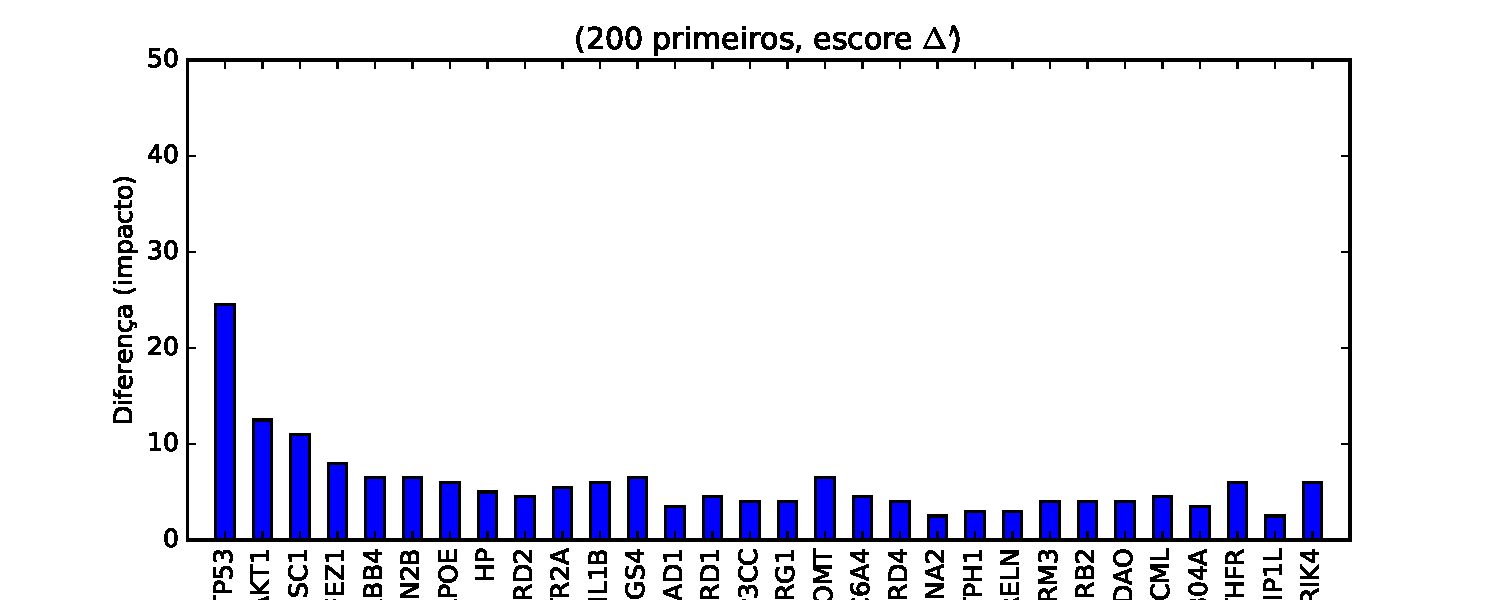
\includegraphics[width=1\textwidth]{Images/analyses/fig_LOO_S_200.pdf}
\caption {Análise dos 100 e 200 primeiros elementos ordenados por $\Delta'$.
\label{fig_LOO_S_100-200}}
\flushleft{Fonte: Produzido pelos autores.}
\end{figure}
%
A imagem \ref{fig_LOO_S_100-200} também apresenta dois gráficos comparativos em relação a similaridade do ranqueamento gênico baseado na quantidade de elementos selecionados. O gráfico de cima, apresenta a diferença em percentual da similaridade dos \textbf{\textit{100}} primeiros genes e o de baixo os primeiros \textbf{\textit{200}}.

%
Podemos observar em ambos os gráficos, que neste ponto de análise não houve remoção de gene que não causou impacto na similaridade dos resultados em relação a amostra original.

%
Um fato importante que ambos os gráficos demonstram, é a mediana dos impactos, onde apresentaram um valor abaixo de \textbf{\textit{10\%}}. Isso demonstra que o impacto gerado pela remoção de um único gene semente varia em torno de \textbf{\textit{10\%}}, o que é muito aceitável em vista da assertividade obtida.

%
Ao observarmos o gene \textbf{\textit{TP53}}, que durante todo o experimento foi o que apresentou maior impacto no resultado, podemos notar que o mesmo apresentou um aumento de \textbf{\textit{17\%}} do impacto para \textbf{\textit{24\%}} ao compararmos os ranqueamentos de \textbf{\textit{100}} e \textbf{\textit{200}} genes. Este valor pode ser considerado baixo, em vista que o numero de elementos da lista analisada foi dobrado e a diferença do impacto gerado foi de \textbf{\textit{7\%}}.

% 
Um comportamento que aparece em ambos os gráficos, que não havia aparecido com tanta nitidez nos anteriores, é a decrescência do impacto da esquerda para direita. Onde os experimentos estão ordenados com relação ao seu grau na rede interna gerada pelo método NERI. Isso implica que mesmo não tendo uma relação direta com o impacto o grau do gene semente apresenta correlação ao analisar uma quantidade maior de genes priorizados do resultado final.

%
%
% ============== X ===============
%
%
\subsection{Estudo dos gráficos em relação ao escore \textit{X}}
%
\subsubsection{Análise dos 10 primeiros elementos}
%
%Imagem
\begin{figure}[ht!]
\centering
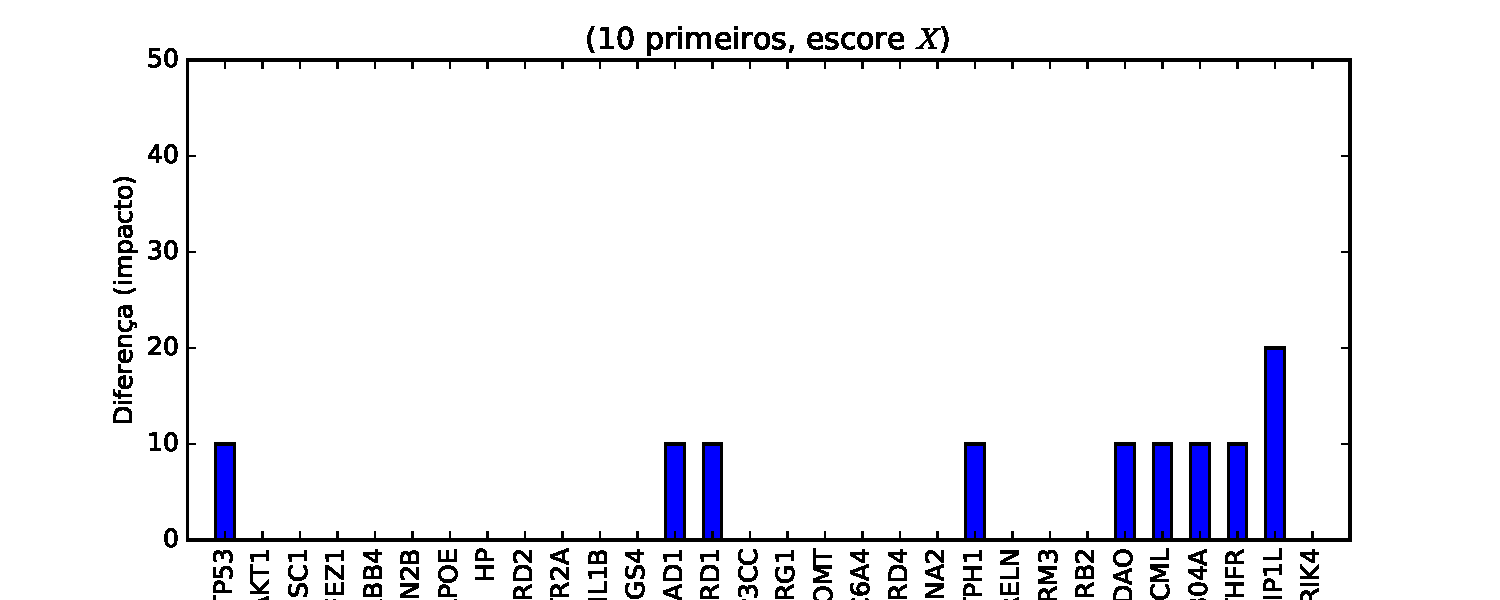
\includegraphics[width=\textwidth]{Images/analyses/fig_LOO_X_10.pdf}
\caption {Análise dos 10 primeiros elementos ordenados por \textit{X}.
\label{fig_LOO_X_10}}
\flushleft{Fonte: Produzido pelos autores.}
\end{figure}
%

%
A figura \ref{fig_LOO_X_10} apresenta um gráfico comparativo referente aos resultados dos experimentos com remoção de apenas \textsl{um gene semente} por vez. O eixo \textbf{Horizontal} representa cada experimento com seu respectivo \textbf{gene semente} removido do agrupamento original, estando estes ordenados  pelo grau que representa na rede gerada pelo método NERI. Sendo esta organização, do maior para o menor no sentido esquerda para direita. O eixo \textsl{Vertical}, por sua vez, representa a \textsl{diferença percentual} dos genes ranqueados em relação ao experimento original, tendo como fator de ordenação o escore \textsl{\textbf{X}}. Por conseguinte, apresentando a comparação dos \textsl{10} primeiros genes ranqueados, sendo estes em relação a remoção do respectivo \textsl{gene semente} apresentado, com os 10 primeiros ranqueados pelo \textsl{experimento original}.
%

Em primeira análise, podemos perceber que o gene semente \textbf{\textsl{RPGRIP1L}} causou o maior impacto em sua remoção, apresentando o percentual de \textsl{\textbf{20\%}} de diferença dos \textsl{\textbf{genes ranqueados}} em relação a amostra original. Este impacto apresenta um comportamento de \textsl{\textbf{outlier}} em relação ao agrupamento de experimentos, em vista que a mediana dos impactos foi de \textsl{\textbf{0\%}}, ou seja, a maior parte dos experimentos em questão não apresentaram diferença entre os \textsl{genes ranqueados} com o \textsl{experimento original}.
%

Podemos observar também que apenas \textsl{\textbf{9}} genes apresentaram impacto em sua remoção. Sendo entre estes, a mediana do impacto \textsl{\textbf{10\%}}, o que é um bom indicador da robustez do método NERI.
%

Um ponto importante para observação é a mudança do gene causador de maior impacto em relação aos \textsl{\textbf{fatores de ranqueamento}}. Quando o ranqueamento foi feito pelo escore \textsl{\textbf{$\Delta'$}} (analisado na seção anterior), o gene semente causador de maior impacto foi \textsl{\textbf{TP53}}, este no qual aprestou apenas \textsl{\textbf{10\%}} de impacto em relação ao escore de ranqueamento \textsl{\textbf{X}}. Isso indica que ambos os genes são impactantes no resultado final do experimento, porém, a abordagem adotada para ranqueamento gênico influencia diretamente na análise.
%


\subsubsection{Análise dos 20 e 50 primeiros elementos}
%
%Imagem
\begin{figure}[ht!]
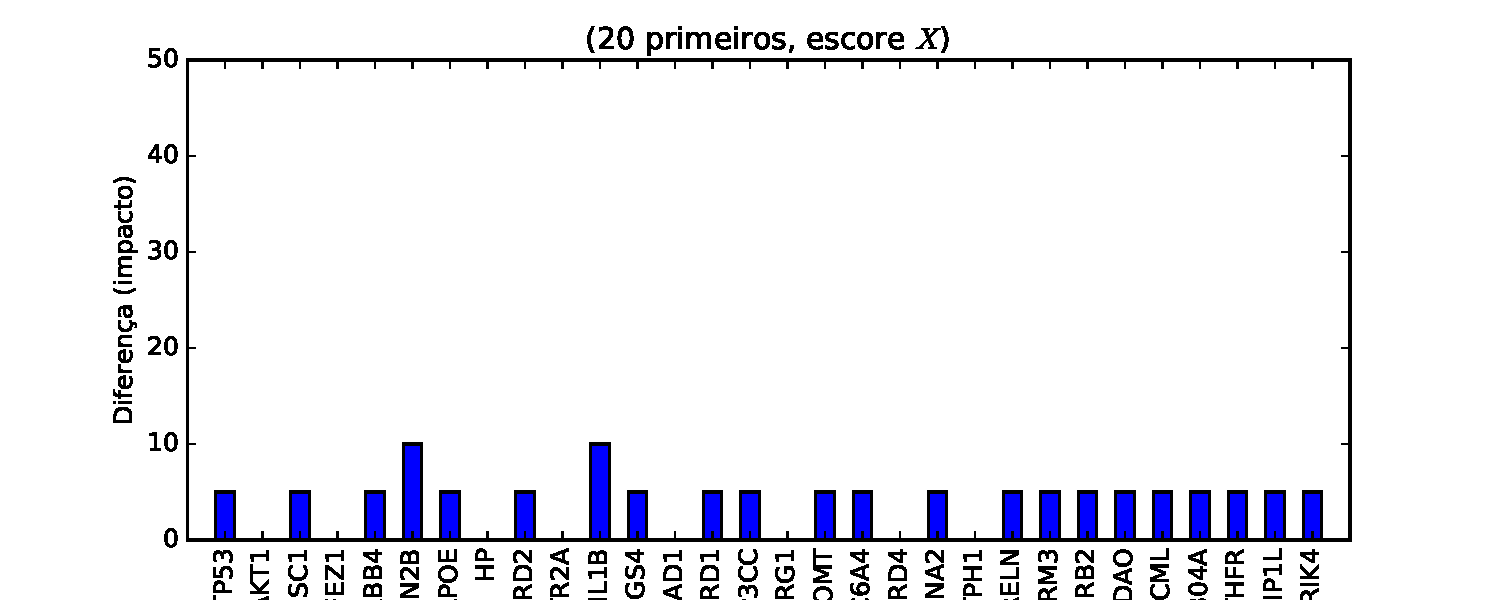
\includegraphics[width=1\textwidth]{Images/analyses/fig_LOO_X_20.pdf}
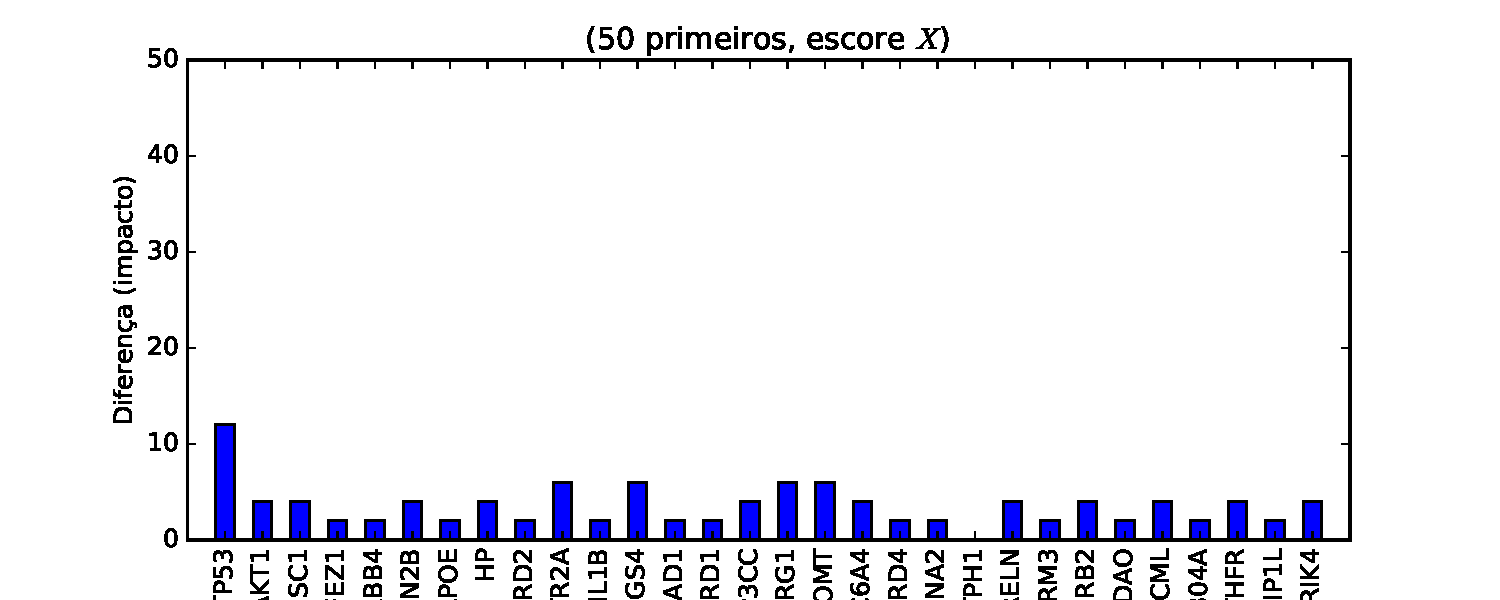
\includegraphics[width=1\textwidth]{Images/analyses/fig_LOO_X_50.pdf}
\caption {Análise dos 20 e 50 primeiros elementos ordenados por \textit{X}.
\label{fig_LOO_X_20-50}}
\flushleft{Fonte: Produzido pelos autores.}
\end{figure}
%

%
A figura \ref{fig_LOO_X_20-50} apresenta dois gráficos comparativos, demonstrando o impacto causado no ranqueamento gênico pelo método NERI ao remover determinados genes sementes. Cada gráfico representa o impacto relativo a quantidade dos genes priorizados analisados, de forma que o eixo \textsl{Horizontal} represente os genes removidos em cada experimento, estando ordenados da esquerda para direita levando em conta grau do gene semente. Assim sendo, o eixo \textsl{Vertical} indica o impacto causado no resultado final em relação a amostra original, este impacto se dá pela diferença percentual de genes presentes no agrupamento experimento e agrupamento original. Estão representados no gráfico de cima, o impacto causado em relação ao ranqueamento dos \textsl{\textbf{20}} primeiros genes, e os \textsl{\textbf{50}} primeiros no gráfico de baixo.

%
Podemos observar em primeira observação, que a quantidade de genes que causaram impacto no ranqueamento gênico. Onde o impacto aumentou consideravelmente logo nos primeiros \textsl{\textbf{20}} genes analisados, sendo \textsl{\textbf{22}} experimentos impactantes. Diferente dos \textsl{\textbf{10}} primeiros, como pode ser visto no gráfico da figura \ref{fig_LOO_X_10}, onde apenas \textsl{\textbf{9}} experimentos apresentaram impacto. Este mesmo comportamento pode ser observado, ao compararmos o gráfico dos \textsl{\textbf{20}} primeiros genes, com o gráfico dos \textsl{\textbf{50}} primeiros. Este ultimo apresenta apenas \textsl{\textbf{1}} experimento que não causou impacto em sua remoção, sendo ele a remoção do gene \textsl{\textbf{TPH1}}.

%
Quando olhamos para o experimento com a remoção do gene \textsl{\textbf{TPH1}}, podemos notar um comportamento atípico. O mesmo apresentou um impacto no ranqueamento gênico de \textsl{\textbf{10\%}} nos primeiros \textsl{\textbf{10}} genes analisados. Porém, nos dois gráficos subsequentes, representando respectivamente \textsl{\textbf{20}} e \textsl{\textbf{50}} primeiros genes ranqueados, o mesmo não apresentou impacto. Ao observarmos este comportamento, podemos inferir que este gene não é de grande importância para o ranqueamento gênico feito pelo método NERI.

%
O gráfico que representa os \textsl{\textbf{20}} primeiros genes ranqueados em relação a \textsl{\textbf{X}}, apresenta uma mediana de impacto de apenas \textsl{\textbf{5\%}}, valor este, considerado muito baixo, em vista que estes são os genes considerados mais importantes pelo método NERI.

%
Uma outra ótica que podemos incutir aos experimentos é a observação em relação ao grau dos genes sementes removidos. Os gráficos demonstram que em relação ao escore \textsl{\textbf{X}}, o grau é um fator altamente impactante no resultado final, em vista que os genes com maior grau \textsl{\textbf{TP53}}, \textsl{\textbf{AKT1}} e \textsl{\textbf{DISC1}} não apresentaram em sua maioria os maires impactos no resultado final. Ficando esta métrica salva apenas para o \textsl{\textbf{TP53}} na análise dos \textsl{\textbf{50}} primeiros genes ranqueados, onde seu impacto é de \textsl{\textbf{22\%}} em relação a amostra original.

%


%
%
\subsubsection{Análise dos 100 e 200 primeiros elementos}
%
%Imagem
\begin{figure}[ht!]
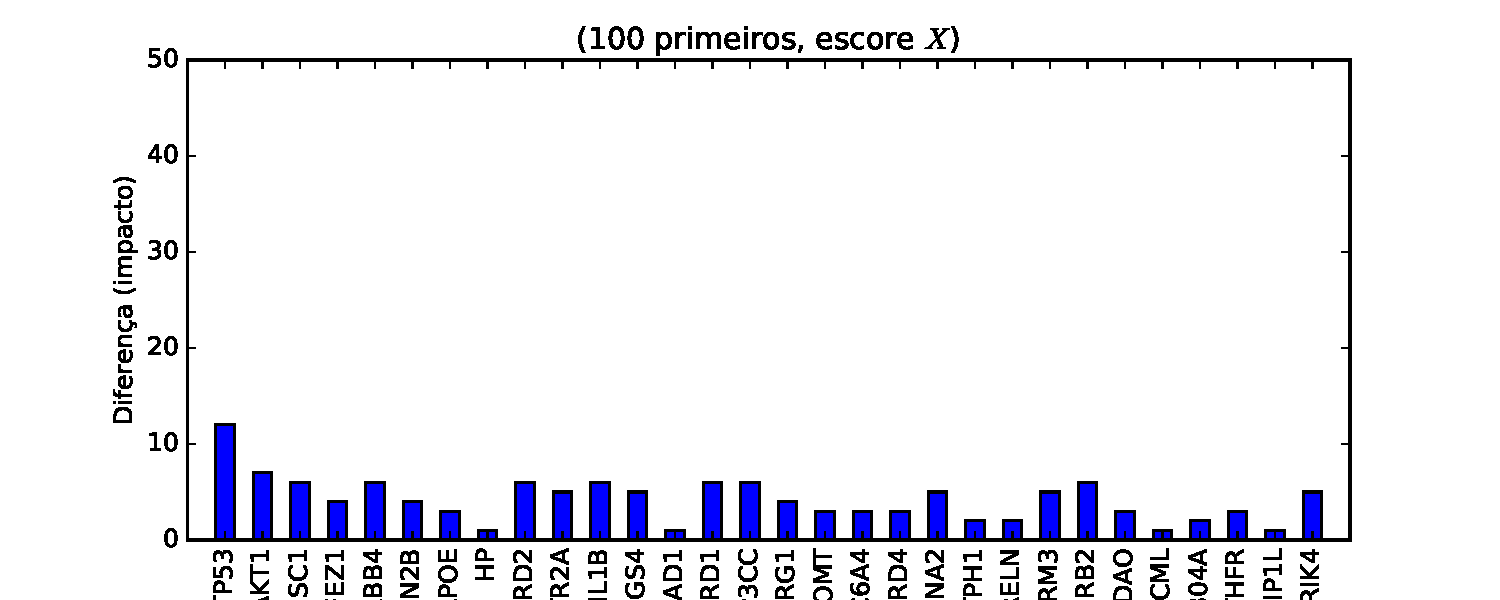
\includegraphics[width=1\textwidth]{Images/analyses/fig_LOO_X_100.pdf}
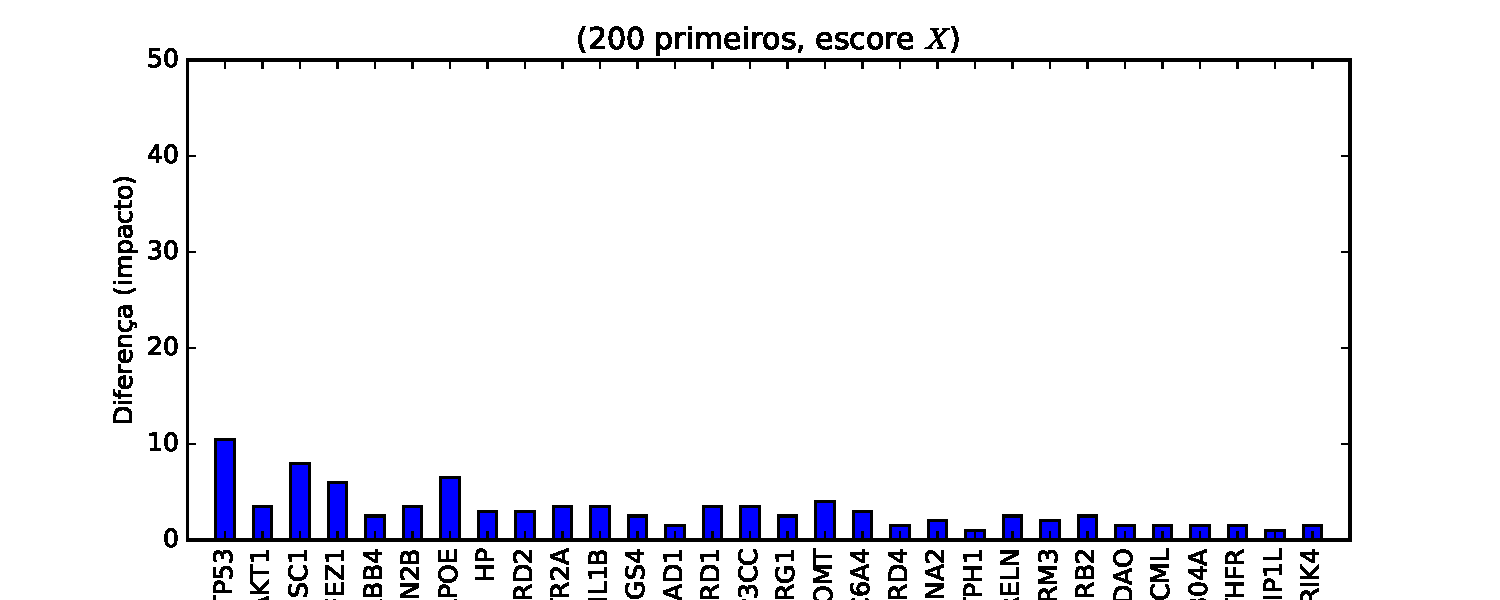
\includegraphics[width=1\textwidth]{Images/analyses/fig_LOO_X_200.pdf}
\caption {Análise dos 100 e 200 primeiros elementos ordenados por \textit{X}.
\label{fig_LOO_X_100-200}}
\flushleft{Fonte: Produzido pelos autores.}
\end{figure}
%
%

A Figura~\ref{fig_LOO_S_100-200} apresenta dois gráficos comparativos em relação ao impacto representado pela remoção do \textsl{\textbf{gene semente respectivo}}. Estes gráficos podem ser lidos da mesma forma que os apresentados anteriormente nesta sessão, onde o de cima representa os primeiros \textsl{\textbf{100}} genes ranqueados e o de baixo os \textsl{\textbf{200}} primeiros.
%

Um comportamento que podemos observar ao analisar os dois gráficos apresentados, é a diminuição do impacto geral causado pela remoção dos genes sementes encontrados nos primeiros \textsl{\textbf{200}} genes ranqueados. Esta diminuição no impacto se dá pelo aumento da lista de genes ranqueados, de forma que mais genes em comum estejam nas listas geradas pelos experimentos e na lista do experimento original. Este comportamento indica uma tendência de diminuição do impacto em relação ao tamanho da lista analisada, porém, o gene semente causador de maior impacto em sua remoção ainda se mantém, sendo \textsl{\textbf{TP53}} com \textsl{\textbf{12\%}} e \textsl{\textbf{10\%}} de impacto nos gráficos de \textsl{\textbf{100}} e \textsl{\textbf{200}} genes ranqueados respectivamente.

Também podemos notar um limiar de impacto abaixo de \textsl{\textbf{10\%}}, ou seja, a maioria dos experimentos causaram um impacto igual ou inferior a \textsl{\textbf{10\%}} no resultado final em relação a remoção do gene semente respectivo. Este comportamento é um bom indicativo para a robustez do método, em vista que o mesmo se mostra com baixa variação no resultado em relação a remoção de um único gene semente, quando o fator de ranqueamento é o escore $X$.

%
%
% ============== OBS ===============
%
%
\subsection{Observações}
%
Em relação ao método de validação de \textit{remoção de um único gene}, o método NERI apresentou bons resultados de robustez. De forma que o maior impacto encontrado pela remoção de um único gene semente foi de \textit{\textbf{40\%}} em relação ao escore $\Delta'$. Porém  a mediana das correlações com o mesmo escore de ranqueamento, foi de \textit{\textbf{20\%}} em relação aos \textbf{\textit{10}} primeiros elementos. Estes valores melhoram ao observar o ranqueamento em relação ao escore $X$, apresentando o maior valor de impacto em \textsl{\textbf{20\%}} com o gene \textsl{\textbf{GRIP1L}}. Fato este que chama atenção por ser um gene semente diferente do maior causador de impacto em relação ao escore $\Delta'$, o gene semente \textsl{\textbf{TP53}}. A mediana de impacto nos primeiros \textsl{\textbf{10}} genes ranqueados pelo escore $X$ foi de \textsl{\textbf{0\%}}, ou seja, a remoção de mais da metade dos genes sementes individualmente não causou impacto no resultado final. Isso significa que os na maioria dos casos os genes ranqueados tanto nos experimentos quanto na amostra original foram os mesmos.

%
% Falar sobre a metrica X também
%

Também deve-se levar em conta que o maior impacto encontrado relação aos \textbf{\textit{200}} primeiros genes selecionados pelo escore $\Delta'$, foi de \textbf{\textit{24\%}} apresentando melhora em relação a análise dos \textbf{\texit{10}} primeiros. A medina apresentou uma queda significativa de \textbf{\texit{20\%}} para \textbf{\textit{5\%}}, o que indica uma convergência de genes selecionados da amostra original com os experimentos. Esse tipo de convergência é esperado com o aumento da quantidade de elementos ranqueados, pois a probabilidade de um gene ser selecionado aumenta proporcionalmente ao tamanho do agrupamento de seleção final. Porém, esta premissa não invalida a eficiência do método em questão, em vista que a quantidade de genes possíveis a serem selecionados é muito maior que a lista dos genes ranqueados.
%
Assim sendo, podemos concluir que o método é robusto em relação a retirada de um único gene semente. Porém, para determinar melhor a robustez do método em análise, há a necessidade de estudar os resultados dos outros modelos de validação empregadas neste trabalho.
%
%
% ======================== CROSS VALIDATION ========================
%
%
\section{Remoção de vários genes sementes}
%
Nesta etapa analisaremos os resultados do método de \textit{Remoção de vários gene sementes}, onde como principal meio de apresentação de dados será o estudo dos gráficos gerados e a discussão de suas interpretações.

\subsection{Esperado}
%
O esperado na utilização do método da \textit{Remoção de mais de um gene} é a capacidade de mapear o impacto causado no resultado final baseado na identificação da quantidade de genes sementes removidos em relação a amostra original. Desta forma observar o impacto causado, a medida que conjuntos de tamanhos diferentes são testados. Com este estudo, podemos aproximar um limiar de confiança no método NERI. Para podermos ter uma análise mais precisa dos resultados, cruzaremos os dados encontrados com os dados gerados pela \textit{Remoção de um único gene}, de forma que consigamos entender melhor o comportamento dos resultados apresentados.
%
%
% ===== S =====
%
%
\subsection{Estudo dos gráficos em relação ao escore $\Delta'$}
%
\subsubsection{Análise dos 10 primeiros elementos}
%
%Imagem
\begin{figure}[ht!]
\centering
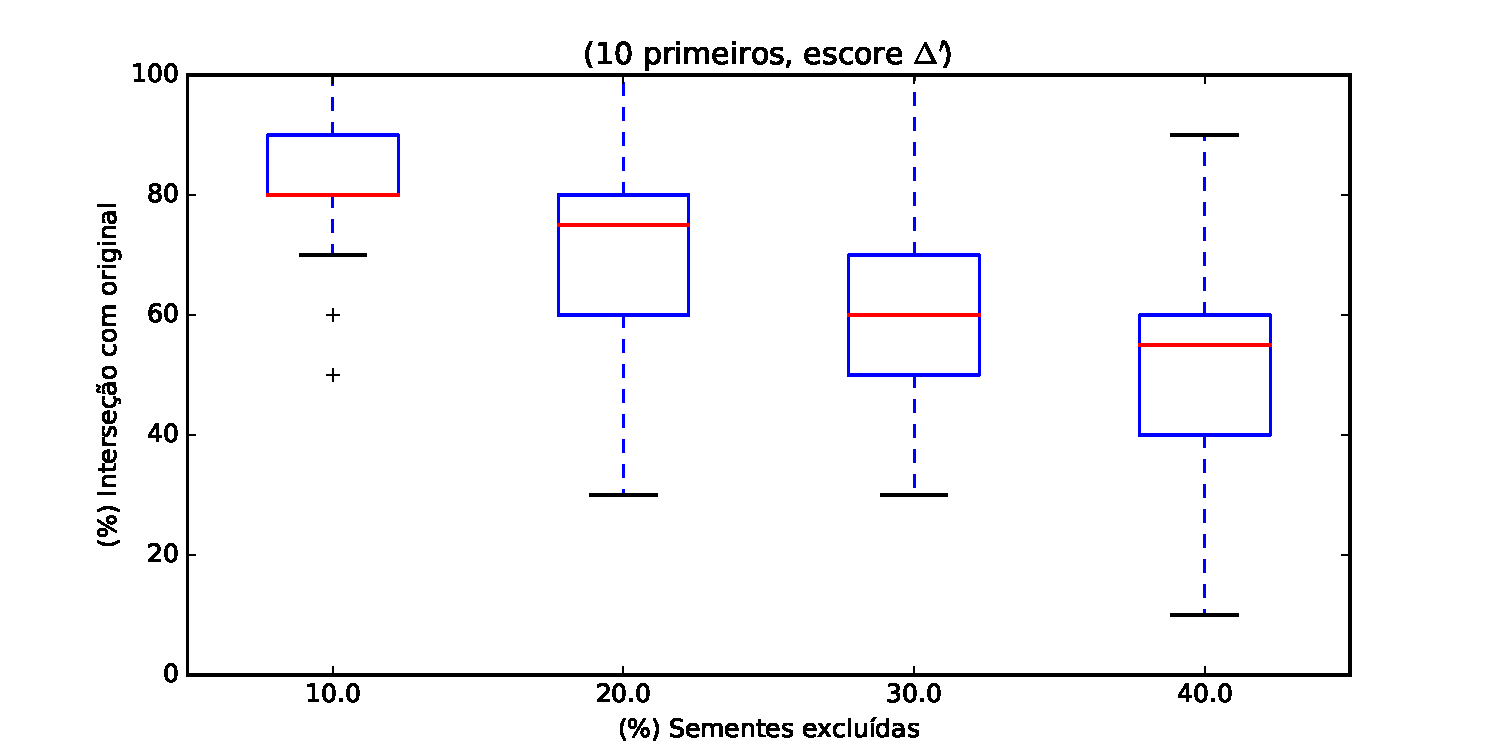
\includegraphics[width=\textwidth]{Images/analyses/fig_S_10_40.pdf}
\caption {Análise dos 10 primeiros elementos ordenados por $\Delta'$.
\label{fig_S_10_40}}
\flushleft{Fonte: Produzido pelos autores.}
\end{figure}
%

%
A Figura~\ref{fig_S_10_40} apresenta um gráfico comparativo dos experimentos utilizando o método \textit{Remoção de mais de um gene}, onde o eixo \textsl{Horizontal} representa a porcentagem de sementes excluídas em relação a amostra original, e o eixo \textsl{Vertical}, por sua vez, representa a porcentagem da interseção dos resultados dos \textsl{\textbf{10}} primeiros genes em relação aos \textsl{\textbf{10}} primeiros apresentados na amostra original, tendo como fator de ranqueamento ao escore $\Delta'$.
%

Conforme podemos observar, a medida que aumentamos o percentual de sementes excluídas, ocorre uma redução gradual na mediana do percentual de interseção de genes selecionados.
Conforme esperado, isso demonstra que a quantidade de genes sementes excluídas influencia diretamente no resultado do experimento.
%

%
Podemos observar também que, a mediana do experimento com a maior porcentagem de remoção apresenta o valor aproximado \textsl{\textbf{50\%}} de interseção, esta métrica é um bom indicativo da robustez do método ao informar que mesmo removendo \textsl{\textbf{40\%}} dos genes sementes, os genes ranqueados pelo método ainda se mantém acima de \textsl{\textbf{50\%}} iguais aos ranqueados pelo método com todos os genes sementes.

Por este gráfico representar somente os \textsl{\textbf{10}} primeiros genes selecionados, esperava-se um impacto no resultado final consideravelmente alto devido ao fato do mesmo apresentar poucos genes em relação ao tamanho da rede \textsl{\textbf{9.554}} Genes (nós). Porém, ao contrário do que imaginávamos, os genes selecionados foram muito próximos da amostra original. Porém a sua precisão varia consideravelmente de modo que a podemos observar que as diferenças entre os limites superiores e inferiores dos experimentos são altas. Isto se dá devido ao tamanho da lista de genes priorizados analisada.
%

Um ponto que chama bastante atenção ao analisar este gráfico, é o boxplot que representa \textbf{\textsl{40\%}} dos genes sementes removidos. O mesmo, apresenta uma variação entre o lime inferior e o limite superior de \textbf{\textsl{60\%}}, ou seja, a bateria de experimentos representados pelo gráfico possui experimentos de similaridade variada entre \textbf{\textsl{20\%}} a \textbf{\textsl{80\%}}. Fato este implica em uma não confiança nos dados representados por este, o comportamento apresentado é reforçado ao fazer uma análise dos \textbf{\textsl{outliers}}. Encontrando um experimento com \textbf{\textsl{90\%}} de similaridade e em contrapartida, um experimento com apenas \textbf{\textsl{10\%}} sendo o menor de todo o estudo em relação aos \textbf{\textsl{10}} primeiros genes removidos.

\subsubsection{Análise dos 20 e 50 primeiros elementos}
%Imagem
\begin{figure}[ht!]
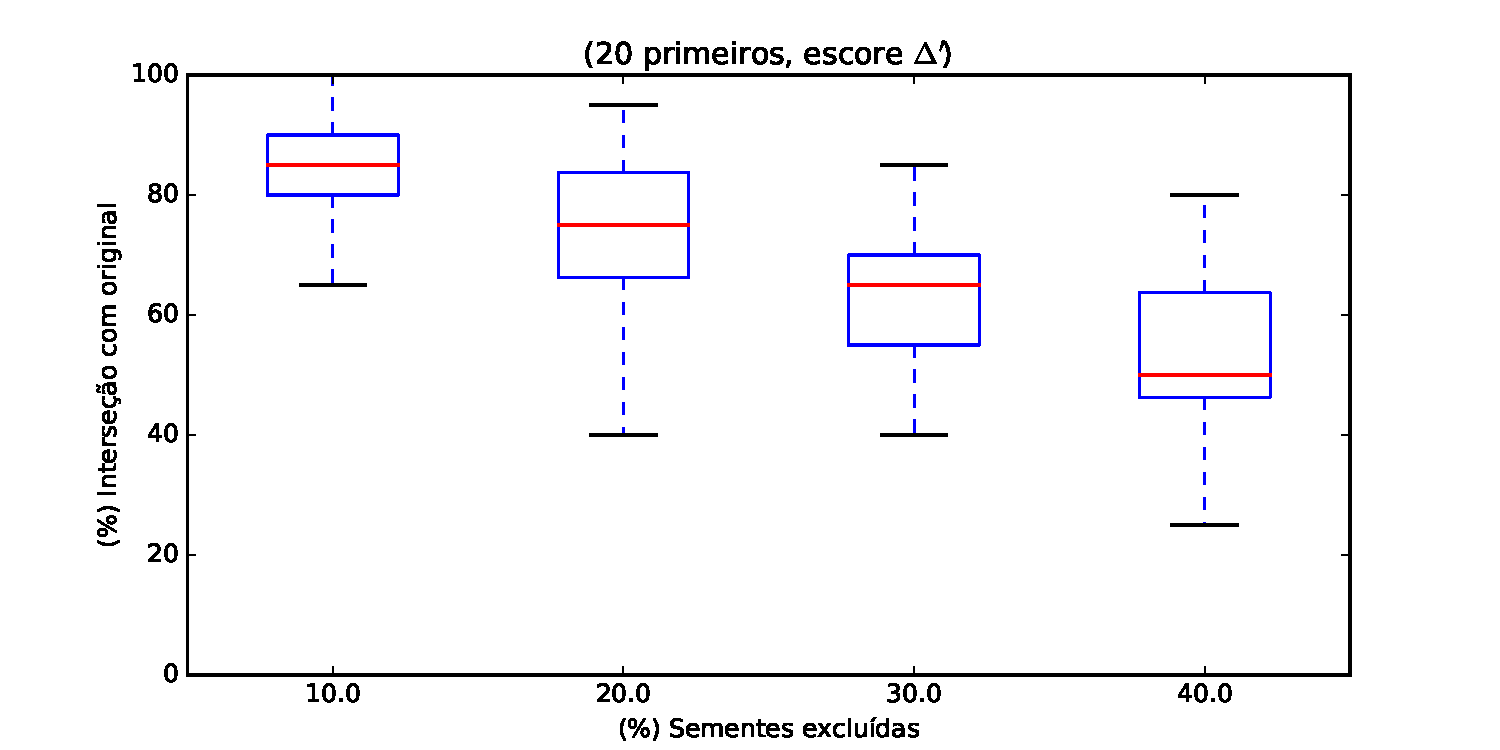
\includegraphics[width=1\textwidth]{Images/analyses/fig_S_20_40.pdf}
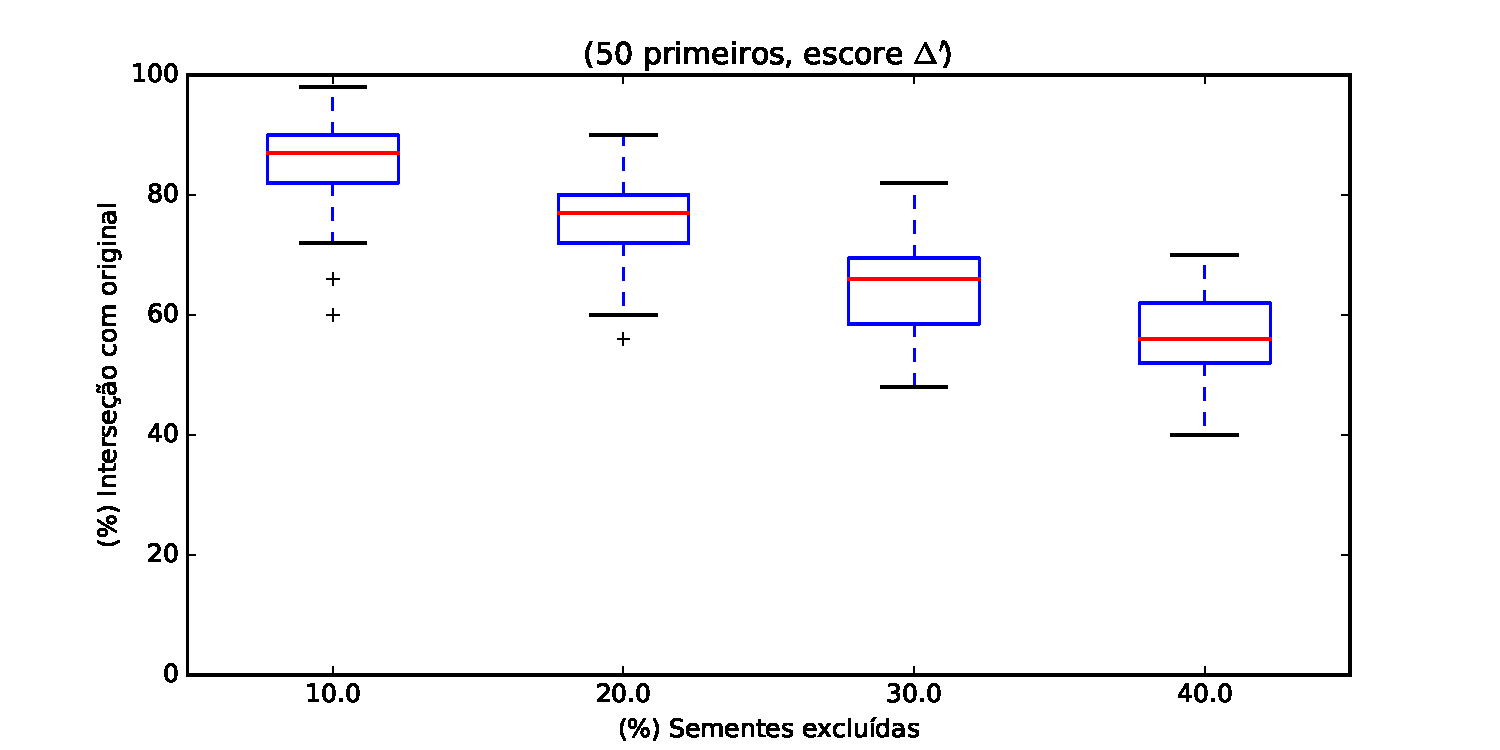
\includegraphics[width=1\textwidth]{Images/analyses/fig_S_50_40.pdf}
\caption {Análise dos 20 e 50 primeiros elementos ordenados por $\Delta'$.
\label{fig_S_20-50_40}}
\flushleft{Fonte: Produzido pelos autores.}
\end{figure}
%

A Figura~\ref{fig_S_20-50_40} apresenta dois gráficos comparativos, sendo o de cima representando a correlação com os \textsl{\textbf{20}} primeiros genes selecionados e de baixo com os primeiros \texit{\textbf{50}}. 
%

Podemos observar no primeiro gráfico a baixa variação da mediana, porém houve uma diminuição na \textit{amplitude interquartílica}. Isto demonstra uma possível convergência de resultados em relação aos dois gráficos. Este fator pode ser observado no \textit{boxplot} referente a \textbf{\textsl{20\%}} do gráfico de cima, onde este representa \textsl{\textbf{20}} primeiros genes selecionados. Neste caso, \textit{amplitude interquartílica} varia de \textit{68\%} a \textit{82\%}, totalizando \textit{14\%} de faixa de variação. No gráfico de baixo, representando os \textbf{\textit{50}} primeiros genes selecionados. Neste caso, há uma variação na \textsl{amplitude interquartílica} de \textbf{\textsl{73\%}} a \textbf{\textsl{80\%}}, totalizando uma faixa de variação de \textbf{\textsl{7\%}}, valor este que apresenta-se metade do valor do gráfico anterior. Esta queda de amplitude remete ao comportamento de convergência, assim representando uma segurança nos resultados apresentados, partindo do princípio de que quanto menor a variação dos resultados, maior é a precisão da medição.
%

Podemos observar também alguns experimentos que ficaram fora do agrupamento, este comportamento é definido como \textit{outlier}. Para entender o porque destes experimentos terem sido apresentados unanimamente com menores resultados do que o corpo amostral, cruzamos os seus dados com os obtidos pela etapa de \textit{remoção de um único gene}. Com este cruzamento de dados, observamos se os genes removidos nestes experimentos contém um ou mais genes que possuem os maiores \textsl{\textsl{graus de impacto}} no resultado.
%

% VERIFICAR QUAIS FORAM OS CASOS DENTRO DO CODIGO
Em 10 experimentos essa premissa apresentou-se verdadeira, resultando menores correlações, onde nestes casos observou-se a falta dos genes sementes \textbf{\textsl{TP53}} e \textbf{\textsl{AKT1}}. Onde ambos causaram o maior impacto no resultado final ao serem removidos sozinhos do experimento (como foi mencionado na sessão anterior). Estes casos apontam uma correlação do impacto acumulativo da remoção de genes sementes no resultado final.
%%%%%
%
%
%
\subsubsection{Análise dos 100 e 200 primeiros elementos}
%
%Imagem
\begin{figure}[ht!]
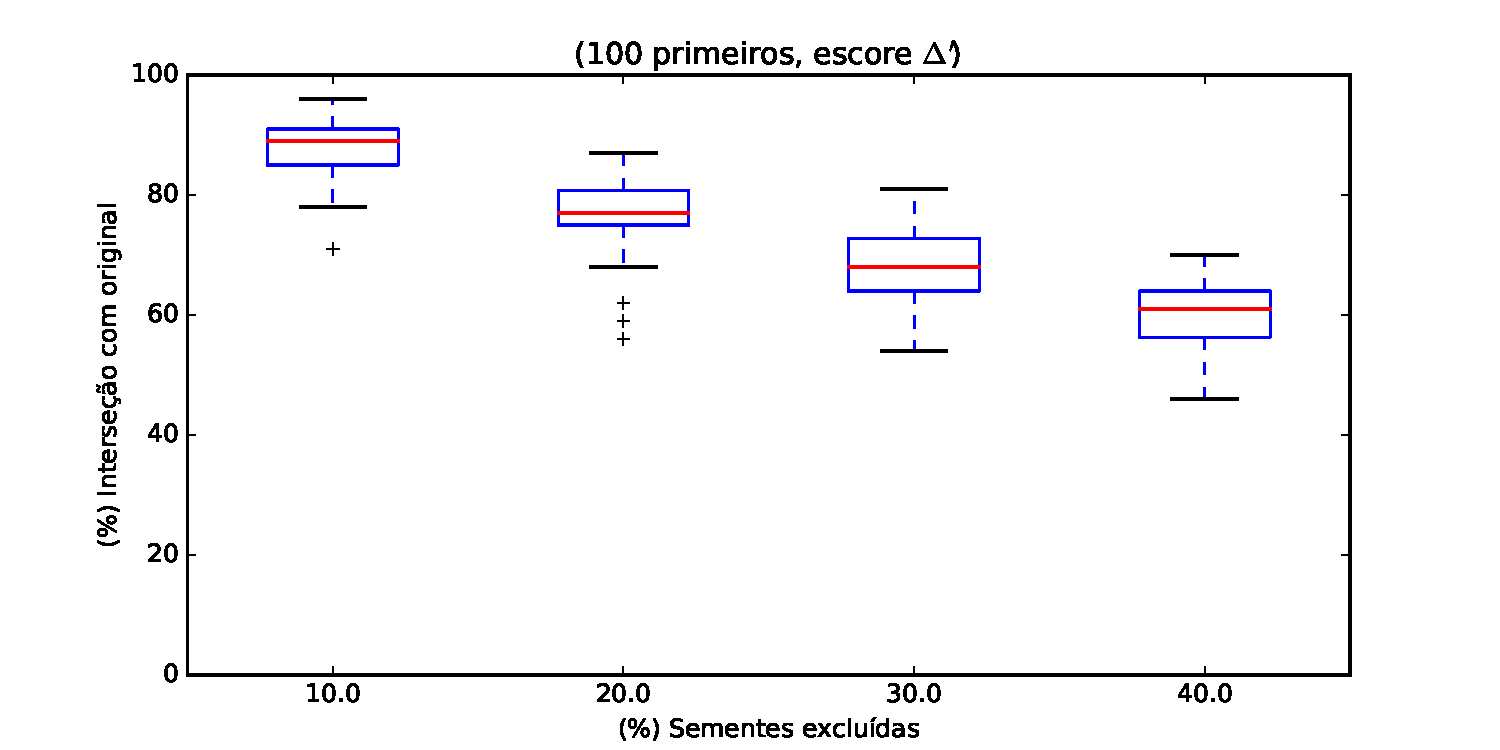
\includegraphics[width=1\textwidth]{Images/analyses/fig_S_100_40.pdf}
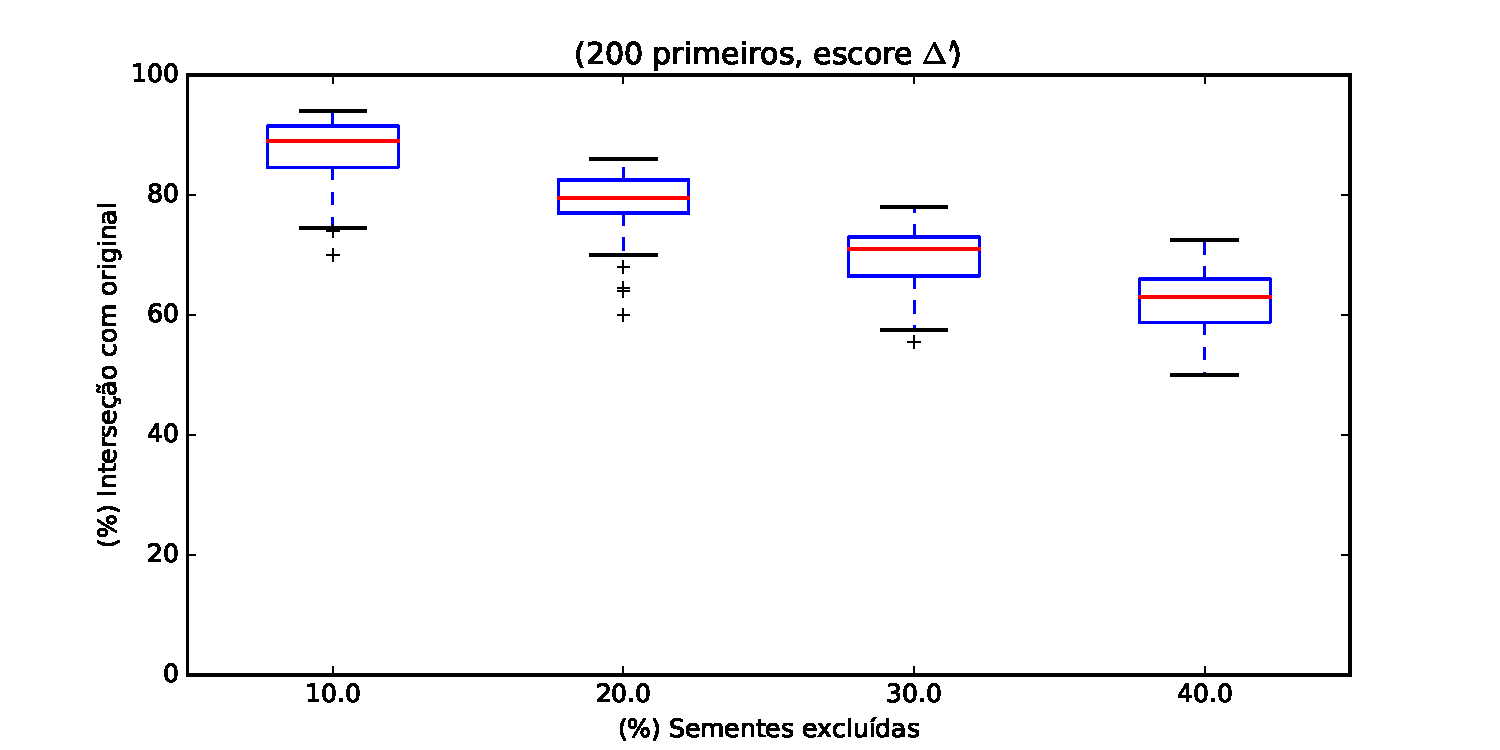
\includegraphics[width=1\textwidth]{Images/analyses/fig_S_200_40.pdf}
\caption {Análise dos 100 e 200 primeiros elementos ordenados por $\Delta'$.
\label{fig_S_100-200_40}}
\flushleft{Fonte: Produzido pelos autores.}
\end{figure}
%%
%

A figura \ref{fig_S_100-200_40} apresenta dois gráficos comparativos entre agrupamentos de experimentos com variação na quantidade de genes sementes. O gráfico \textsl{de cima}, representa a comparação dos \textsl{\textbf{100}} primeiros genes ranqueados em relação ao escore $\Delta'$, onde o eixo \textsl{Horizontal} define os \textsl{boxplots} correspondentes as suas determinadas porcentagens de retirada dos \textsl{\textbf{genes sementes}}. Assim sendo, o eixo \textsl{Vertical} define a porcentagem de interseção dos genes ranqueados pelos experimentos em relação ao experimento original.
Seguindo esta mesma organização, o gráfico \textsl{de baixo} representa os \textsl{\textbf{200}} primeiros genes ranqueados.
%

Podemos notar claramente, que o decrescimento correlacional está presente nos dois gráficos. Ou seja, a correlação dos \textsl{\textbf{genes ranqueados}} cai em mesma proporção nos dois gráficos conforme a quantidade de \textsl{\textbf{genes sementes}} são reduzidas. Porém, podemos enxergar que a \textsl{\textbf{amplitude interquartílica}} respectiva entre os gráficos apresenta uma diminuição. Este aspecto representa bons resultados, pois indica que há uma convergência de resultados conforme o aumento dos \textsl{\textbf{genes ranqueados}} observados.
%

Nesta comparação, podemos observar novamente comportamentos de \textsl{\textbf{outlier}} presentes nos gráficos. Como na análise anterior, os agrupamentos que apresentaram menor correlação, foram os que não tinham em seu agrupamento de \textsl{\textbf{genes sementes}} os mais impactantes observados na etapa de \textsl{\textbf{retirada de uma único gene semente}}, sendo eles \textsl{\textbf{TP53}} e \textsl{\textbf{AKT1}}.
%

Um forte fator de análise é a comparação entre o gráfico dos \textsl{\textbf{10}} primeiros genes ranqueados (\ref{fig_S_10_40}) com o gráfico dos \textsl{\textbf{100}} (\ref{fig_S_100-200_40}). Podemos observar que a mediana subiu de \textsl{\textbf{80\%}} de correlação com a amostra original, para \textsl{\textbf{90\%}} ao comparar os \textsl{\textbf{boxplots}} pertencentes a \textsl{\textbf{10\%}} de remoção. Este fato aponta para uma robustez do método analisado, em vista que fortalece ainda mais o efeito de convergência observado anteriormente. Ao comparar com o gráfico dos \textsl{\textbf{200}} genes ranqueados, notamos que a \textsl{\textbf{mediana}} se mantém a mesma em relação a dos \textsl{\textbf{100}}, indicando que esta convergência ocorre entre nos primeiros \textsl{\textbf{100}} genes ranqueados, sendo este um número muito bom. O mesmo pode ser observado ao comparar os outros \textsl{\textbf{boxplots}} respectivos, os valores apresentados não são os mesmos, mas apresentam um padrão muito próximo de variação.



%
%%%%%
%
%
% ===== X =====
%
%
\subsection{Estudo dos gráficos em relação ao escore \textit{X}}
\subsubsection{Análise dos 10 primeiros elementos}
%
%Imagem
\begin{figure}[ht!]
\centering
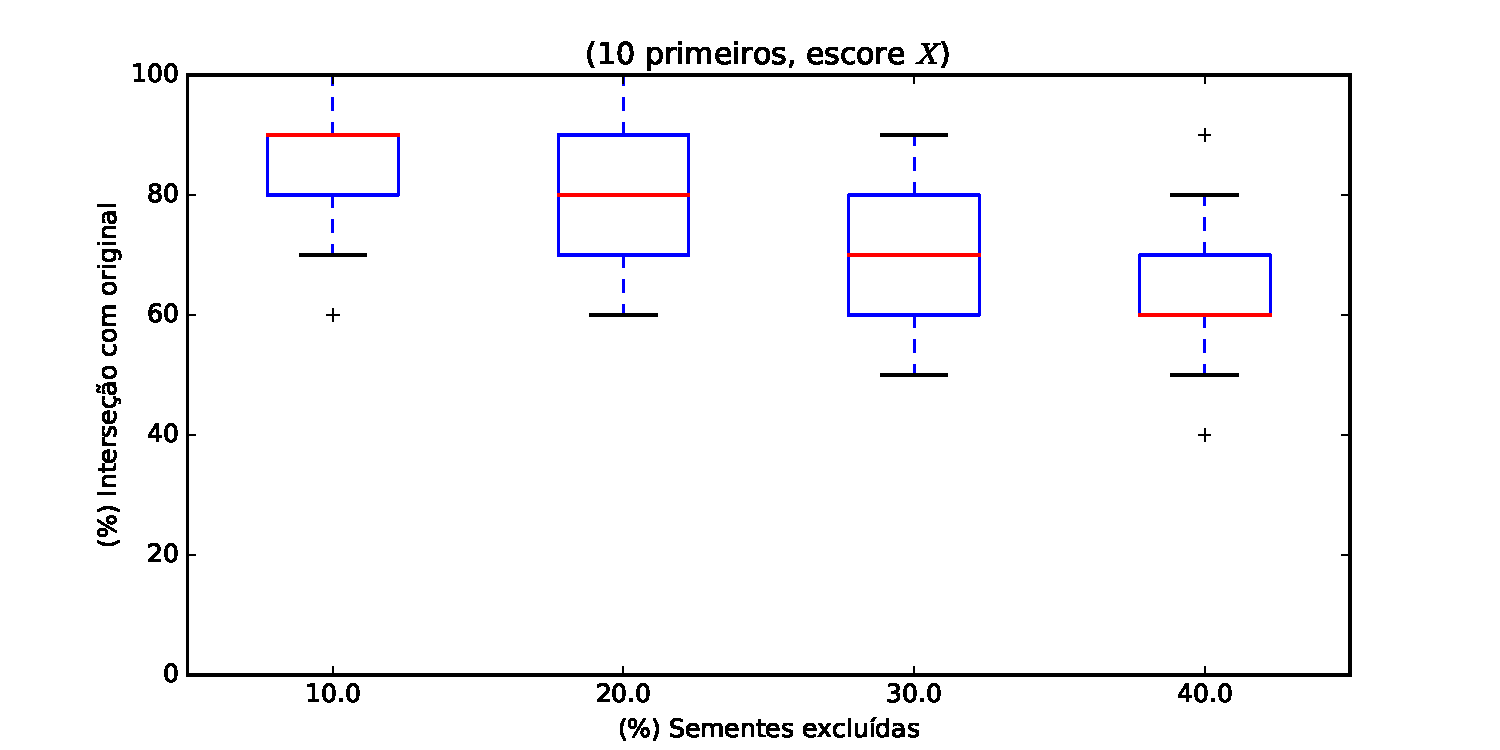
\includegraphics[width=\textwidth]{Images/analyses/fig_X_10_40.pdf}
\caption {Análise dos 10 primeiros elementos ordenados por \textit{X}.
\label{fig_X_10_40}}
\flushleft{Fonte: Produzido pelos autores.}
\end{figure}
%
%

%
A Figura~\ref{fig_X_10_40} apresenta um gráfico comparativo dos experimentos utilizando o método \textit{Remoção de mais de um gene}, onde o eixo \textsl{Horizontal} representa a porcentagem de sementes excluídas em relação a amostra original, e o eixo \textsl{Vertical}, por sua vez, representa a porcentagem da interseção dos resultados dos \textsl{\textbf{10}} primeiros genes em relação aos \textsl{\textbf{10}} primeiros apresentados na amostra original, tendo como fator de ranqueamento o escore $X$.
%
Em primeira análise, fica claro que, assim como o ranqueamento pelo escore de ranqueamento $\Delta'$, quanto maior a quantidade de genes sementes removidos nos experimentos, a correlação das listas de priorização gênica diminui. Fator este esperado, em vista que o método NERI utiliza os genes sementes para realizar a priorização gênica.
%

Ao compararmos este gráfico com o apresentado na análise do escore $\Delta'$ como pode ser vista na Figura~\ref{fig_S_10_40}, podemos notar que a variação dos resultados dos experimentos é muito menor, indicando que o escore $X$ tende a ser mais robusto. O boxplot que intuitivamente apresentaria maior diferença de limite superior e inferior, o referente a \textbf{\textsl{40\%}} de remoção de genes sementes, não apresentou uma grande variação. Este comportamento é o contrário do observado anteriormente, onde a variação anterior apresentou-se em \textbf{\textsl{60\%}}, diferentemente do gráfico em relação ao escore \textbf{$X$} apresentando \textbf{\textsl{30\%}}, metade do valor anterior. Sugerindo mais uma vez a robustez do escore de ranqueamento $X$ superior ao escore $\Delta'$.

Podemos notar que a mediana do pior caso ficou em \textbf{\textsl{60\%}} de similaridade com a lista de genes ranqueados em relação ao experimento original. O pior caso sendo determinado intuitivamente pelo conjunto de experimentos com  \textbf{\textsl{40\%}} de remoção dos genes sementes em relação ao experimento original. A variação entre a menor e maior mediana, sendo elas respectivamente \textbf{\textsl{60\%}} e \textbf{\textsl{90\%}}, apresenta-se em \textbf{\textsl{30\%}}. Um valor muito bom se levarmos em consideração que no pior caso foram removidos \textbf{\textsl{40\%}} dos genes sementes da amostra original, ou seja, a variação do impacto proporcional causado foi menor que o fator de remoção de genes sementes em relação a amostra original. Isto indica uma boa robustez do método NERI em relação ao fator de ranqueamento $X$.  

\subsubsection{Análise dos 20 e 50 primeiros elementos}
%
%Imagem
\begin{figure}[ht!]
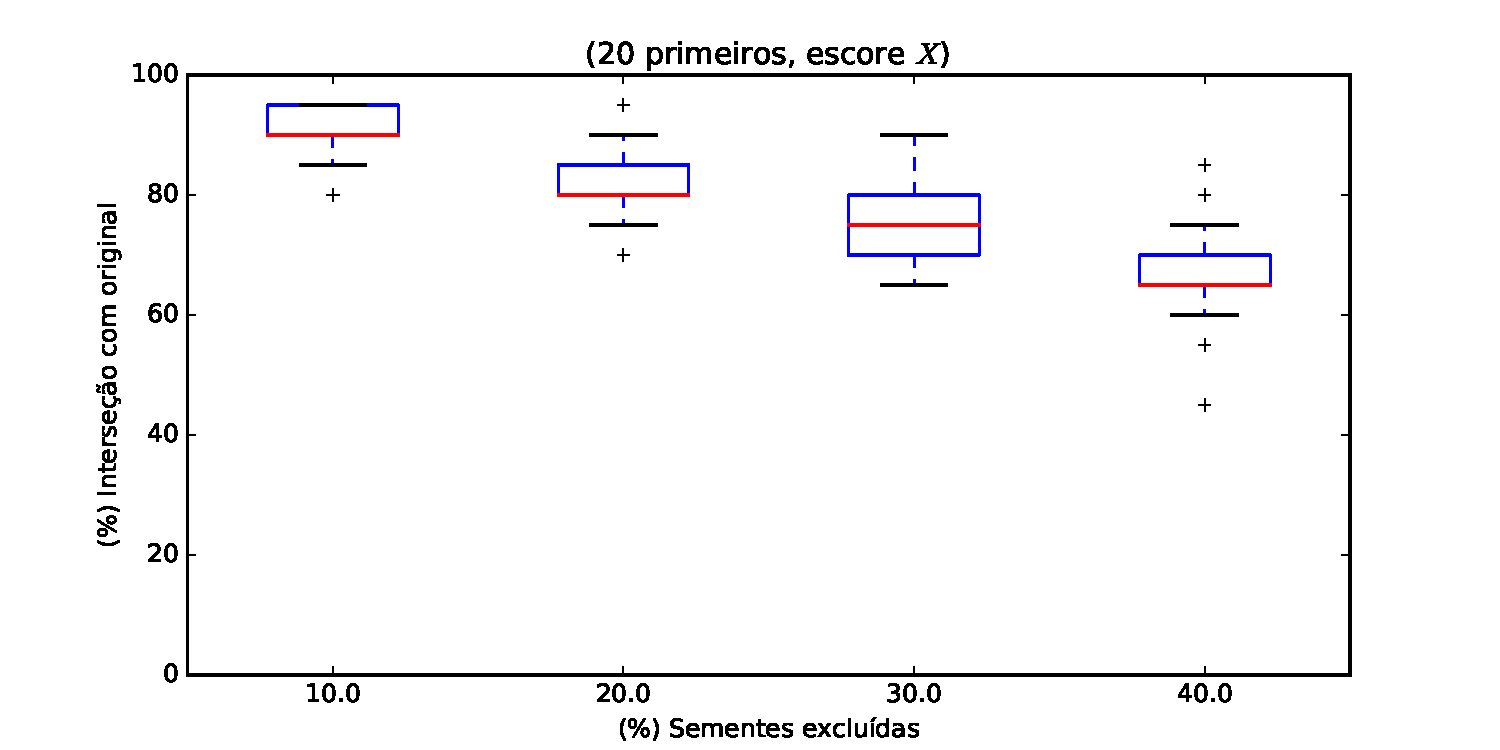
\includegraphics[width=1\textwidth]{Images/analyses/fig_X_20_40.pdf}
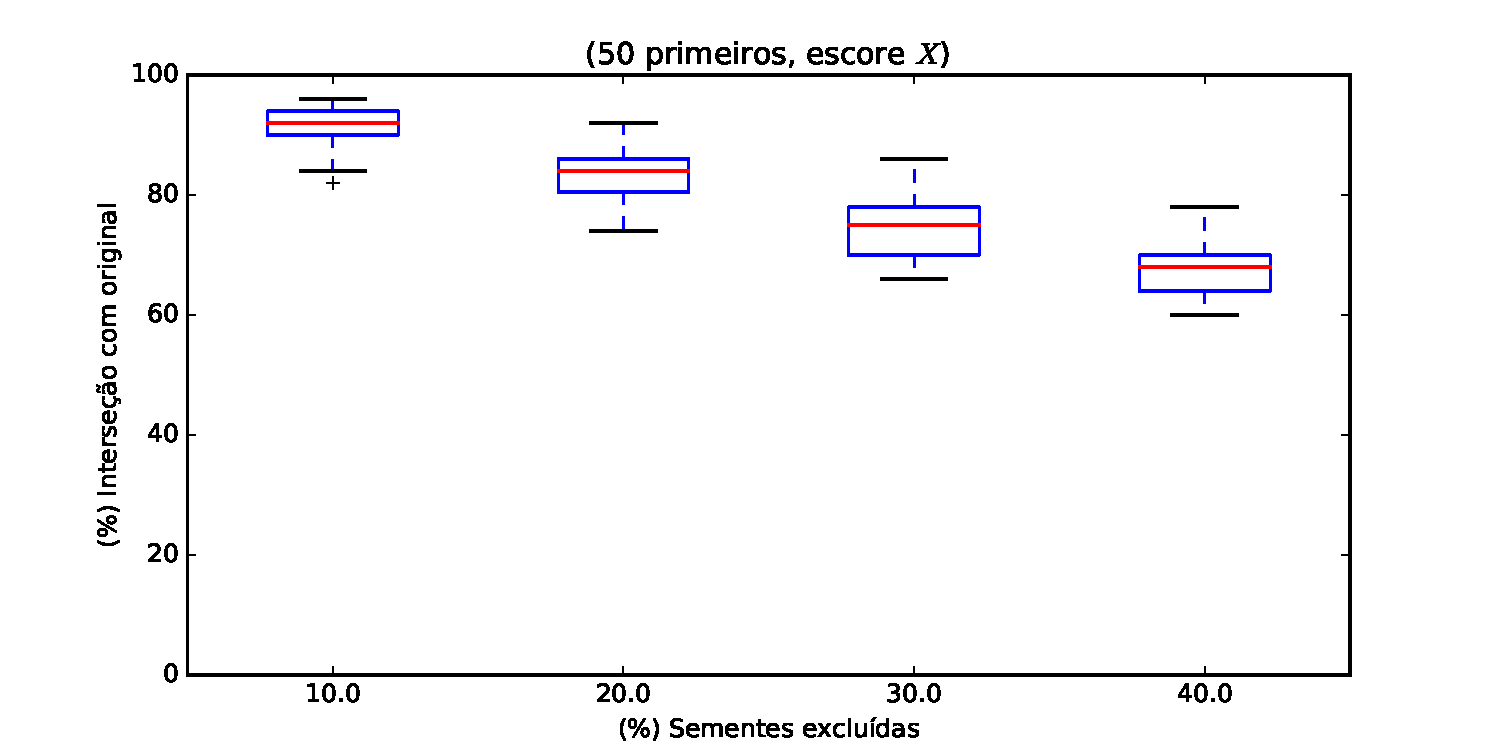
\includegraphics[width=1\textwidth]{Images/analyses/fig_X_50_40.pdf}
\caption {Análise dos 20 e 50 primeiros elementos ordenados por \textit{X}.
\label{fig_X_20-50_40}}
\flushleft{Fonte: Produzido pelos autores.}
\end{figure}
%

%
A Figura~\ref{fig_X_20-50_40} apresenta dois gráficos comparativos dos experimentos utilizando o método \textsl{Remoção de mais de um gene}, onde o gráfico de cima representa os \textsl{\textbf{20}} primeiros genes ranqueados pelos experimentos e o de baixo os primeiros \textsl{\textbf{50}}. Ambos no eixo \textsl{Horizontal} apresentam as porcentagens de genes sementes removidos em relação a amostra original e no eixo \textsl{Vertical}, a porcentagem de similaridade do resultado dos experimentos com o resultado original, ou seja, a similaridade das listas dos experimentos em relação a lista de ranqueamento gênico original.
%

Pode-se notar que, as amplitudes amostrais diminuíram em ambos os casos, isso demonstra uma menor variação dos experimentos em relação a análise feita dos \textsl{\textbf{10}} primeiros genes. Este comportamento, era intuitivamente esperado, em vista que ao aumentar a quantidade de genes selecionados na lista de ranqueamento, a probabilidade da variação dos resultados diminuírem aumenta. Porém, como são muitos genes na rede, o aumento de \textsl{\textbf{10}} e \textsl{\textbf{40}} genes ranqueados em relação a análise anterior, foi o suficiente para identificação. Apesar de ter sido esperado, representa um bom sinal de robustez, de modo que a baixa variação do resultado seja um fator para a mesma.
%

Nota-se também que no gráfico que representa os \textsl{\textbf{20}} primeiros genes ranqueados, quando analisou-se os experimentos que tiveram \textsl{\textbf{40\%}} dos genes sementes removidos em relação a amostra original, apresentaram experimentos \textsl{\textbf{ouliers}} onde alguns representavam uma boa correlação e outros uma má correlação. Isto indica que devemos observar os genes presentes nestes experimentos, para assim tentarmos entender o comportamento diferenciado. Os experimentos \textsl{\textbf{outliers}} que apresentaram uma má correlação, tiveram entre os seus genes sementes removidos os seguintes elementos \textsl{\textbf{TP53}} e \textsl{\textbf{RPGRIP1L}}. Estes genes sementes, são os que apresentaram um maior impacto em sua remoção única na etapa de \textsl{Remoção de um único gene}, onde podemos correlacionar que, o impacto mostra-se acumulativo, ou seja, se um gene com alto impacto em sua remoção é removido juntamente com outro gene causador de um alto impacto, ambos aumentam o impacto total da amostra em questão. Já os experimentos que apresentaram boa correlação, apresentaram a remoção de genes sementes que não causaram grande impacto em sua remoção na etapa de \textsl{Remoção de um único gene}, sendo exemplo destes os elementos \textsl{\textbf{GAD1}} e \textsl{\textbf{HP}}, estes que apresentaram um impacto sempre abaixo de \textsl{\textbf{10\%}}.   
%

Ao observar as medianas dos experimentos, pode-se enxergar que há uma diminuição conforme aumenta a quantidade de genes sementes removidos em relação ao experimento original. Este aspecto indica uma dependência do método NERI aos genes sementes, fato este já sabido previamente, devido ao mesmo valer-se destes genes para o ranqueamento gênico. O que chama a atenção é o fato da proporção de remoção ser menor que a proporção de impacto causado, ou seja, ao remover \textsl{\textbf{40\%}} dos genes sementes, não impacta o resultado em \textsl{\textbf{40\%}}, mas sim em menos, no caso dos \textsl{\textbf{20}} e \textsl{\textbf{50}} primeiros genes ranqueados, este impacto fica em torno dos \textsl{\textbf{35\%}}.



%
\subsubsection{Análise dos 100 e 200 primeiros elementos}
%
%Imagem
\begin{figure}[ht!]
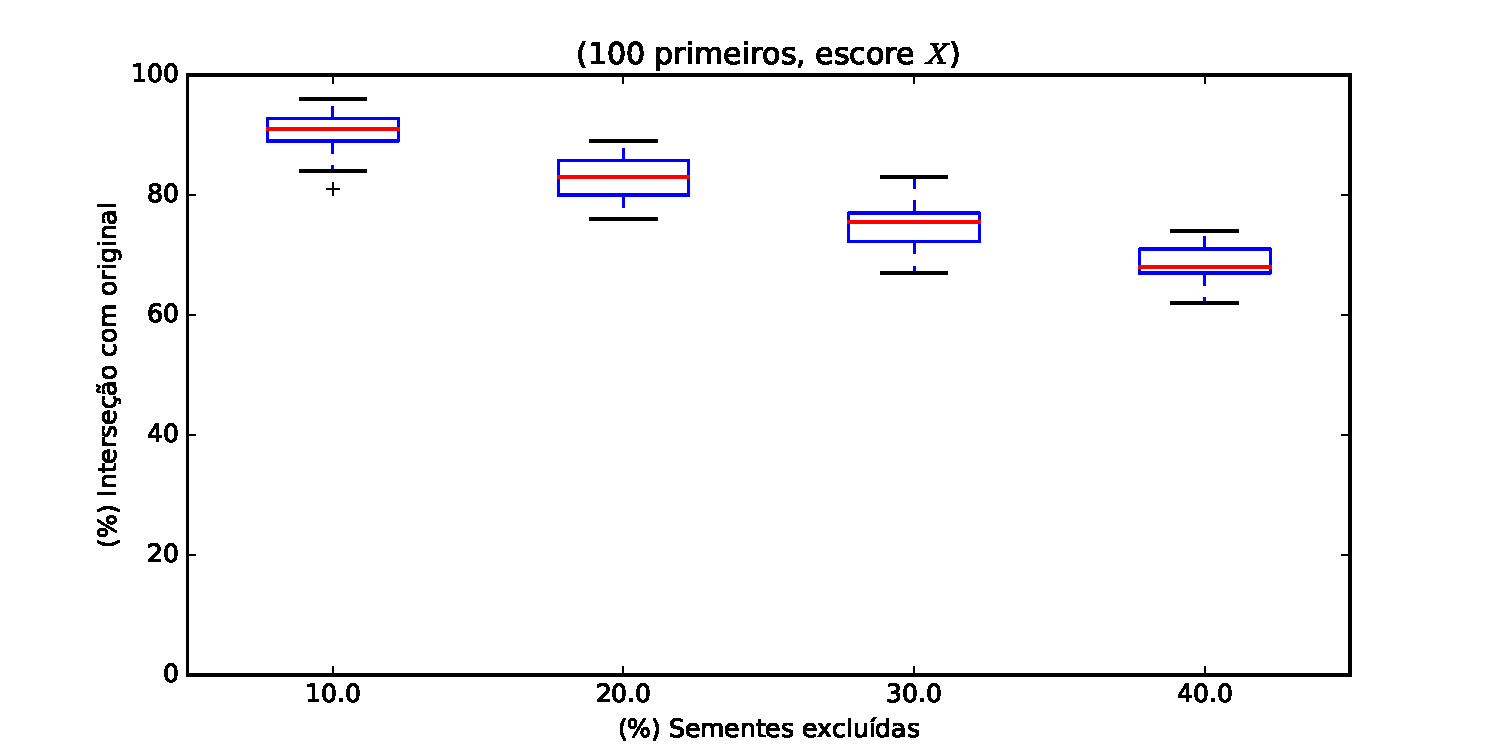
\includegraphics[width=1\textwidth]{Images/analyses/fig_X_100_40.pdf}
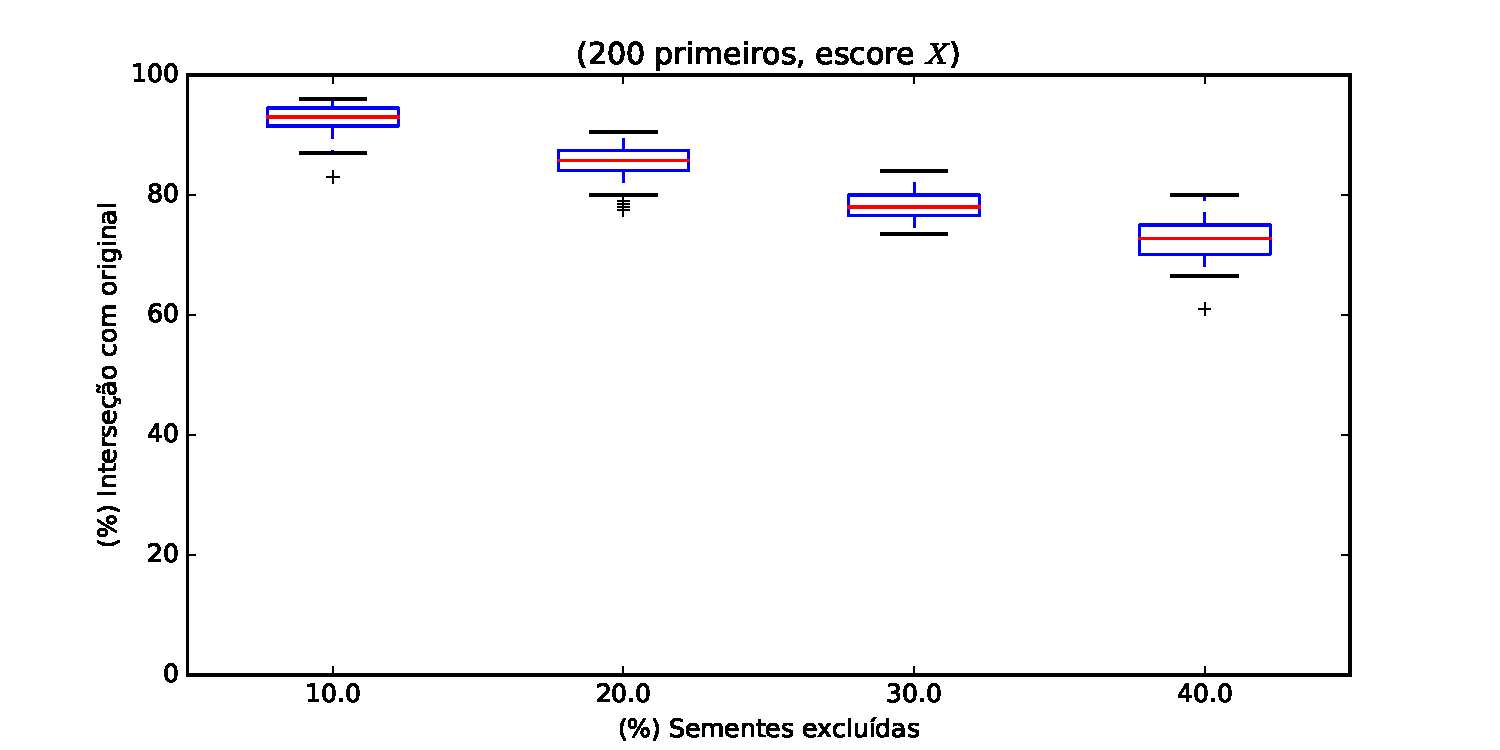
\includegraphics[width=1\textwidth]{Images/analyses/fig_X_200_40.pdf}
\caption {Análise dos 100 e 200 primeiros elementos ordenados por \textit{X}.
\label{fig_X_100-200_40}}
\flushleft{Fonte: Produzido pelos autores.}
\end{figure}
%%
%

%
A Figura~\ref{fig_X_100-200_40} apresenta dois gráficos comparativos em relação aos experimentos que foram gerados através do método \textsl{Remoção de mais de um gene}, onde o gráfico de cima representa os \textsl{\textbf{100}} primeiros genes ranqueados pelos experimentos e o de baixo os primeiros \textsl{\textbf{200}}. Ambos no eixo \textsl{Horizontal} apresentam as porcentagens de genes sementes removidos em relação a amostra original e no eixo \textsl{Vertical}, a porcentagem de similaridade do resultado dos experimentos com o resultado original, ou seja, a similaridade das listas dos experimentos em relação a lista de ranqueamento gênico original.
%

%
Podemos notar que mesmo os \textsl{outliers} presentes em ambos os gráficos apresentam uma boa correlação com o experimento original. Isto afirma que todos experimentos executados apresentaram um bom resultado de replicabilidade ao analisar os primeiros \textbf{\textsl{100}} e \textbf{\textsl{200}} genes priorizados pelo método NERI. Este aspecto indica uma forte robustez do método, em vista que mesmo os experimentos que apresentaram comportamento diferente do conjunto no qual estão inseridos obtiveram uma boa correlação com o experimento original.

%
Outro aspecto importante para se observar é o comportamento das correlações dos experimentos, quanto maior a quantidade de genes sementes removidos da amostra original, menor a correlação obtida com o experimento original. Este comportamento esteve presente em todas as análises feitas, tanto no escore $X$ quanto no $\Delta'$, comprovando a dependência do método NERI em relação aos genes sementes. Porém mesmo assim, apresentou-se robusto a remoção dos genes sementes, indicando bons resultados de replicabilidade. Fato este que torna a utilização do método analisado mais confiável. 
%

%
\subsection{
\label{sec:compXS}
Comparação do escore $X$ com o escore $\Delta'$}
%

Podemos notar que o escore $X$ é mais robusto em relação a remoção de genes sementes se comparado com o escore $\Delta'$, apresentando menor variação nos resultados e um menor impacto no resultado final em relação a amostra original. Um fator impactante é a comparação das Figuras~\ref{fig_X_10_40} (\textsl{\textbf{10}} primeiros genes ordenados pelo score $X$) e \ref{fig_S_10_40} (\textsl{\textbf{10}} primeiros genes ordenados pelo score $\Delta'$), onde podemos observar a diferença das correlações nos \textsl{boxplots} referentes a \textsl{\textbf{40\%}} de remoção dos genes sementes em relação a amostra original. O \textsl{boxplot} que representa a ordenação pelo score $\Delta'$ apresenta uma amplitude amostral onde o valor mínimo representado é de aproximadamente \textsl{\textbf{10\%}} de similaridade com a amostra original, valor este que apresenta-se muito baixo se comparado com o \textsl{boxplot} que representa a ordenação pelo score $X$ onde o valor mínimo apresentado é por um experimento com comportamento \textsl{outlier} e corresponde a \textsl{\textbf{40\%}} de similaridade com a amostra original. Outra métrica observada é a amplitude amostral de ambos, ainda observando o pior caso (\textsl{\textbf{40\%}} de remoção dos genes sementes em relação a amostra original), onde o score $X$ apresenta \textsl{\textbf{30\%}} de variação contra \textsl{\textbf{80\%}} apresentado pelo score $\Delta'$.
%

%
As variações dos resultados e a amplitude interquartílica dos \textsl{boxplots} apresentam-se maiores em $\Delta'$ em todas as análises comparativas entre aos dois escores. Isto indica novamente uma maior confiabilidade em termos de variação de resultado no score $X$. Este comportamento se dá pela natureza dos scores, onde o score $X$ é baseado na soma de todas as medidas de centralidade calculadas pelo método NERI e o score $\Delta'$ é baseado nas pontuações condicionais da rede, fato este que ao faltar um determinado gene semente que representaria algum papel na rede, o score condicional apresenta variação. Sendo assim, uma forma de ranqueamento gênico menos confiável que o embasamento no score $X$. Este fato não invalida a utilização da mesma, em vista que esta apresentou bons resultados em linhas gerais, onde o impacto no resultado final em pouquíssimos casos ficou acima de \textsl{\textbf{50\%}} (em casos de extremo estresse, como na remoção de \textsl{\textbf{40\%}} dos genes sementes em relação a amostra original e observando o apenas os \textsl{\textbf{10}} primeiros genes ranqueados).
%

\section{Desempenho computacional}
%\textcolor{red}{======= REESCREVER DAQUI P BAIXO =======}

%Podemos considerar que o método tende a ser robusto ao observar os top 10 primeiros genes selecionados, levando em conta seu comportamento em relação a remoção de genes sementes do experimento, porém ainda não podemos tirar conclusões concretas sem antes observar sob outras perspectivas os resultados dos experimentos, como por exemplo, o espalhamento dos resultados em relação ao eixo Y de cada agrupamento, existem amostras que apresentaram resultados muito discrepantes em relação ao conjunto no qual ele pertence.
%Para estudar estes casos, alguns aspectos devem ser analisados, sendo um deles, quais genes foram removidos e quais não foram, isso permitirá um melhor entendimento do comportamento dos \textsl{outliers}.



Os fatores envolvidos no processo de execução dos experimentos, foram as configurações da máquina no qual foi executada e a disponibilidade de tempo execução.
As configurações da maquina no qual foram executados os experimentos são as descritas abaixo:

\begin{itemize}
    \item \textbf{Processador:} \textsl{i7} geração 5.
    \item \textbf{Memória:} 16 GB - 2 pentes 8GB DDR3 1600Ghz.
    \item \textbf{Armazenamento:} 50 GB HD disponíveis.
\end{itemize}

 
Pelo fato do programa que implementa o método NERI ainda não utilizar paralelismo (utilização de mais de um núcleo de processamento), foram executadas 4 instâncias separadas ao mesmo tempo, durante todo a etapa de execução do experimento.

\subsection{Consumo de Processamento}
Cada instância ocupou 100\% de processamento de um núcleo físico presente no processador, como a máquina utilizada possui 4 núcleos físicos e foram executadas 4 instâncias simultaneamente, o consumo de cpu foi para 100\% do total presente.

\subsection{Consumo de Memória}
Cada instância em execução consumiu em média 1,5 GB de memória, totalizando aproximadamente 6 GB alocados por todas as 4 instâncias executantes.

\subsection{Utilização de disco}
Devido ao fato de os experimentos serem executados em modo \textsl{Debug}, a escrita em arquivo dos \textsl{logs} foi realizada durante boa parte do tempo de execução.
Isto significa que, se os modo \textsl{Debug} for desabilitado, os tempos podem ser um pouco menores.
Os 30 experimentos ocuparam aproximadamente 6,5 MB; para a remoção de um único gene foram realizados 30 experimentos (um para cada semente); e para a remoção de vários genes foram realizados 50 experimentos para cada percentual de remoção (10\%, 20\%, 30\% e 40\%), totalizando $50 x 4 = 200$ experimentos de remoção de vários genes.
Desta forma, os 230 experimentos realizados ocuparam aproximadamente 1,2 GB de armazenamento no disco rígido.
